% What Language Labels Leave Out. Compile with xelatex, bibtex, xelatex, xelatex.
\documentclass[final]{clv2025}
\usepackage{fontspec}
% Fonts are loaded by file name so that the build does not depend on the
% system font registry: TeX Gyre ships with TeX Live, and FreeSerif with its
% gnu-freefont package. Name-based lookup is the fallback.
\defaultfontfeatures{Ligatures=TeX}
\IfFontExistsTF{texgyrepagella-regular.otf}
  {\setmainfont{texgyrepagella}[Extension=.otf,UprightFont=*-regular,BoldFont=*-bold,ItalicFont=*-italic,BoldItalicFont=*-bolditalic]
   \setsansfont{texgyreheros}[Extension=.otf,UprightFont=*-regular,BoldFont=*-bold,ItalicFont=*-italic,BoldItalicFont=*-bolditalic]
   \setmonofont{texgyrecursor}[Extension=.otf,UprightFont=*-regular,BoldFont=*-bold,ItalicFont=*-italic,BoldItalicFont=*-bolditalic,Scale=0.92]}
  {\setmainfont{TeX Gyre Pagella}\setsansfont{TeX Gyre Heros}\setmonofont{TeX Gyre Cursor}[Scale=0.92]}
\IfFontExistsTF{Noto Serif Devanagari}
  {\newfontfamily\devfont{Noto Serif Devanagari}[Script=Devanagari]}
  {\IfFontExistsTF{FreeSerif.otf}
    {\newfontfamily\devfont{FreeSerif.otf}[Script=Devanagari]}
    {\newfontfamily\devfont{FreeSerif}[Script=Devanagari]}}
\newcommand{\dev}[1]{{\devfont #1}}
\usepackage{amsmath,amssymb,booktabs,graphicx,array,longtable}
\usepackage{microtype,xurl,etoolbox,placeins}
\hypersetup{hidelinks,
  pdftitle={What Language Labels Leave Out: An Absorbing Class in Corpus Language Identification},
  pdfauthor={Romin Oli},
  pdfsubject={Language identification; corpus construction; Hindi; Angika},
  pdfkeywords={language identification, corpus audit, GlotLID, Hindi, Angika, FineWeb-2},
  pdflang={en}}
\jyear{2026}\jvol{}\jnum{}
\jinfo{Research manuscript}
\dochead{}
\runningtitle{An Absorbing Class in Corpus Language Identification}
\runningauthor{Oli}
\renewcommand{\footmark}{}
\newcommand{\lab}[1]{\texttt{#1}}
\newsavebox{\exhibitbox}
\newcommand{\fitexhibit}[1]{\sbox{\exhibitbox}{\input{#1}}\ifdim\wd\exhibitbox>\linewidth\resizebox{\linewidth}{!}{\usebox{\exhibitbox}}\else\usebox{\exhibitbox}\fi}
\newcommand{\exhibit}[1]{\fitexhibit{tables/#1.tex}}
\graphicspath{{figures/}}
\emergencystretch=1.5em
\hbadness=2500
\raggedbottom
\begin{document}
\title{What Language Labels Leave Out:\\An Absorbing Class in Corpus Language Identification}
\author{Romin Oli}
\affilblock{\affil{Swar Nepal\\\email{oliromin@gmail.com}}}
\maketitle
\pagestyle{pageonly}\thispagestyle{pageonly}
\begin{abstract}
Language identification decides which texts enter a language's share of a multilingual training collection. Inspecting that collection shows what reached a label; it cannot show what the same language lost to other labels. The two views can diverge very far. Across three releases of one identifier, Hindi retention on 2,000 Wikipedia sentences falls from 99.4\% to 48.0\%, while the last release's Hindi-labelled bucket remains 97.8\% Hindi-sourced on the same mixture, and a separate blinded sample shows the loss occurring on text that readers confirm as Hindi. We argue that the two results are readings of one decision region, and that the region brings almost no precision the preceding release lacked. Adding an Angika source row to the evaluation mixture separates the identifiers by where they send it. Those that route most of it to Hindi lose up to 34 percentage points of bucket precision; those that route it elsewhere, to neighbouring labels or to Angika itself, lose far less. The immediately preceding release, which has no Angika class, reaches 0.972 destination composition against the new release's 0.976 while retaining 0.942 of Hindi against 0.480: four thousandths of precision separate the two releases, and 46 percentage points of Hindi retention. The loss is concentrated in the one class rather than spread across the release's other changes: the Hindi cell sends 0.5075 of its units to a class new in version 3 against no more than 0.0160 for any control cell, and 56 of the 61 control units that do move go to Angika. Source, unit length, prior exposure to the evaluated text, register, and confidence filtering each fail to remove or account for the loss. Corpus language-ID audits should therefore be bidirectional, and should measure a new fine-grained class on both sides of the decision it makes.

\end{abstract}

\section{Introduction}

When language identification precedes corpus construction, its decisions shape the data available for NLP training. The audit that follows is almost always an inspection of the resulting collection, and an inspection of a collection is structurally incapable of answering the question that matters most to a language's speakers. It reveals what reached a label. It cannot reveal what was sent elsewhere. A Hindi-labelled collection can therefore be inspected, found precise, and still be missing half of the Hindi that was offered to it.

The asymmetry is not a subtlety of estimation; it is an identity. On a fixed input collection with $N_\ell$ texts in each validated source-language cell, let $T_{m,c}(\ell,j)$ be the fraction of cell $\ell$ that model $m$ assigns to label $j$ under input condition $c$. The number of texts reaching label $j$ before any later filtering is
\begin{equation}\label{eq:identity}
B_j=\sum_\ell N_\ell\,T_{m,c}(\ell,j).
\end{equation}
Nothing about $B_j$, and nothing about the purity of its contents, determines the original supply $N_j$ or the retained fraction $T_{m,c}(j,j)$. An auditor who holds only the collection holds only $B_j$.

We show how far apart the two sides can be. On 2,000 Wikipedia-derived Hindi sentences, GlotLID v1 retains 1,987 as Hindi and v3 retains 960. Yet v3's Hindi-labelled bucket is 97.8\% Hindi-sourced on the same six-language evaluation mixture. High destination precision coexists with a loss of more than half the source. The outcome is not a law: v1 and v2 are high on both measures in that mixture.

Our central claim is that the precision and the loss are two readings of one decision region, and that a comparison with the preceding release shows how little precision accompanies the loss. Version~3 is the only evaluated release carrying an Angika label, and it routes 50.8\% of these Hindi sentences to it. Adding Angika to the source side of the mixture as a seventh language shows how much of that bucket's purity depends on the label. Identifiers that route most of the Angika row to Hindi see their buckets collapse: \lab{lid.176} falls from 0.723 to 0.427 and \texttt{langid.py} from 0.828 to 0.487. Identifiers that route it elsewhere, to neighbouring labels or to Angika itself, hold up. GlotLID v2, which carries no Angika label, reaches 0.972 against v3's 0.976 while retaining 0.942 of Hindi against 0.480 (Section~\ref{sec:seven}). The clean Hindi bucket does not depend on the Angika class: a release without it matched the bucket to within four thousandths while losing about 6\% of Hindi rather than 52\%. What accompanies the class is the loss. Section~\ref{sec:absorbing} assembles the evidence that its decision region absorbs Hindi rather than competing with it at a boundary.

The release changed more than one label, so the class has to be separated from the rest of the change. Version 3 emits 302 labels that version 2 does not, but 157 of those are \lab{und\_} placeholders for unseen Unicode categories, leaving 145 genuine new classes, seven of them Devanagari. Measuring how much of each reference cell version 3 routes to any of the 145 separates the mechanism from release drift, and the result is not diffuse: the Hindi cell sends 0.5075 of its units to a class new in the release, and no other cell sends more than 0.0160. Nor does it look like a general cost of finer resolution. Of the 61 units the five control cells do send to a new class, 56 receive Angika---all of Sanskrit's and all of Newari's among them, although neither is a closely related modern variety whose separation from Angika would explain the routing---while the six other new Devanagari classes take five units between them.

A separate blinded Hindi/Nepali verification sample shows the loss on text that people have judged. Among 279 Hindi units whose provenance label is confirmed by reader~1, v3 retains 216 and assigns 59 to Angika; nine of the 86 Hindi units confirmed by both readers also receive Angika. The two kinds of evidence do different work. The reader judgments establish that the routing failure occurs on independently confirmed Hindi; the larger provenance panels characterize its magnitude under specified source conditions. Neither substitutes for the other.

Five candidate explanations of the loss are measured and none removes it. Prior exposure to the evaluated text does not: 1,554 of the 2,000 panel sentences appear verbatim in the identifier's published Hindi training file, and v3 retains 0.478 of those against 0.487 of the rest, a present-minus-absent difference of $-0.008$ with a source-clustered interval of [$-0.063$, $0.043$]. Register does not: the Wikipedia and news cells are close on function-word evidence, rare-token rate, and stub-template share, and reweighting the news cell to the Wikipedia cell's distribution of any of these absorbs none of the 0.325 source gap (Section~\ref{sec:register}). Proximity to the absorbing class's own training material accounts for about a ninth of it and no more (Section~\ref{sec:ngram}). Unit length delimits the loss without removing it, and the source contrast survives holding the eligible documents fixed across nested lengths. Confidence filtering does not repair it: 574 of the 1,015 Wikipedia sentences assigned to Angika score at least 0.9 and so survive every threshold the published rule permits. A contemporary comparison with OpenLID-v3 shows that severe Hindi loss is not shared by every recent identifier.

We then use released FineWeb-2 partitions to ask what identifier comparisons can tell us about an existing corpus. Two verified GlotLID releases assign Hindi to about 98--99\% of the Angika-labelled documents but seldom to marker-selected Angika controls, and the contrast persists across six shared sentence-length bins. The Awadhi-labelled partition behaves differently. These readings are diagnostics of identifier behaviour, not evidence of either partition's linguistic composition, which neither model agreement nor removal counts can establish.

The contribution is therefore primarily empirical: a measured case in which the release that adds a fine-grained class keeps a label's purity while losing about half of its coverage, on reader-confirmed text, with no filter or covariate we measured removing the loss. The methodological part is smaller and we treat it as such. Section~\ref{sec:design} separates four quantities that corpus audits conflate---source retention, routing destination, destination composition, and the assignment rate a classifier produces on an artifact nobody has annotated. The last is the one corpus audits report in place of a composition estimate, and we use it to keep released-partition readings from being read as one. The experiments do not isolate the cause of the release difference or establish which binary made every historical corpus-production decision.

\section{Related work}\label{sec:related}

Multilingual corpus audits already document language-identification failures and contamination from related languages. \citet{caswell-etal-2020-language} study the difficulties of constructing a thousand-language web corpus, and \citet{kreutzer-etal-2022-quality} assess the usability of language-labelled datasets. MADLAD-400 combines broad coverage with document-level auditing \citep{kudugunta-etal-2023-madlad}. Building on these audits, we examine source retention and destination composition for the same identifiers, keeping the input conditions explicit.

FineWeb-2 addresses contamination from high-resource neighbours through language-specific precision filtering, in addition to confidence and quality filters \citep{penedo2025fineweb2}. GlotCC applies the same identifier family to a broad-coverage crawl corpus and reports its own subcorpus audit \citep{kargaran-etal-2024-glotcc}. Community annotation of FineWeb-2 partitions has already found some of them to be largely another language, with wrong-language rates of 60\% and 78\% of the annotated units in the Swiss German and Ligurian cells \citep{vanstrien2025fineweb}; that work annotates what arrived and is the kind of evidence a destination reading cannot supply on its own. We examine the published confidence rule and two released partitions, while leaving the role of individual production stages unresolved. Language contamination can affect downstream model capabilities \citep{blevins-zettlemoyer-2022-language}, which is why data selection is worth measuring on its own terms; the present experiments measure selection and not downstream performance.

Closely related language identification has a long history \citep{jauhiainen-etal-2019-automatic}. The 2018 Indo-Aryan Language Identification task covers Hindi, Awadhi, Bhojpuri, Braj, and Magahi \citep{zampieri-etal-2018-language}; its leading system achieved 0.958 macro F1 \citep{jauhiainen-etal-2018-iterative}. That curated, restricted-label task differs from our broad-inventory routing evaluation. We retain its original train, development, and test divisions because their Hindi source profiles differ.

The evaluated identifiers include \texttt{langid.py} \citep{lui-baldwin-2012-langid}, CLD3 \citep{cld3}, fastText \lab{lid.176} \citep{joulin2016bag,joulin2016fasttextzip}, OpenLID \citep{burchell-etal-2023-open}, and GlotLID \citep{kargaran-etal-2023-glotlid}. OpenLID-v3 revises training data, variant groupings, and noise handling, with detailed case studies of related languages \citep{fedorova-etal-2026-openlid}. What such a classifier separates languages by is itself under revision: \citet{meister-etal-2026-language} identify language through language-conditional segmentation over a shared tokenizer vocabulary rather than through fixed character n-grams, and report the largest gains on exactly the closely related varieties at issue here. We add the public OpenLID-v3 release to selected central cells, using both common and recommended preprocessing, while preserving the historical releases needed for the version comparison.

CommonLID emphasizes human verification and the gap between conventional benchmarks and web data \citep{ortizsuarez-etal-2026-commonlid}. Our study complements it by following Hindi routing across historical releases and source conditions, using an existing reader-checked sample and a nested-source experiment.

Recall against a released corpus is not a new question. \citet{dent-etal-2025-identifying} measure how much French-based Creole material the released MADLAD-400, GlotCC and FineWeb-2 partitions retain, and report how far a mining pipeline can recover what identifiers and filters left out. The direction is the difference. There the language at risk is the low-resource one being mined, and the competitor for its text is a high-resource neighbour; here it is the high-resource language whose text is taken by a newly added low-resource label. Both are the same side of Equation~\ref{eq:identity} and neither is answered by inspecting a bucket.

Because several of our reference cells are Wikipedia-derived, the provenance of small Wikipedia editions bears directly on how far our source comparisons can be read. \citet{tatariya-etal-2026-good} audit Wikipedia data quality across low-resource and multilingual editions and document how far small editions depart from the running prose their use as training and evaluation material presumes, a concern \citet{kreutzer-etal-2022-quality} raise for language-labelled collections generally. That literature supplies a specific and testable account of our own Wikipedia--news contrast: small-edition Wikipedia text is disproportionately formulaic stub material, dense in proper nouns and thin in the function-word evidence an identifier can use, so an identifier might lose Wikipedia sentences for reasons of register rather than of language. Section~\ref{sec:register} measures that account directly and does not find support for it in these cells, so the source contrast is reported as a contrast between collections and not as a register effect; Section~\ref{sec:ngram} then finds a small part of it elsewhere.
\section{Design and measurement}\label{sec:design}

\subsection{Four different quantities}

Equation~\ref{eq:identity} says that an auditor holding a collection holds $B_j$ and not $N_j$. Recovering the other side requires measuring on the source side of the routing decision, which in turn requires keeping four quantities apart. Three of them are the familiar contents of a confusion table and we define them only to fix notation; the fourth is the one that corpus audits report in place of a composition estimate.

For identifier $m$, let $f_m(x)$ be its predicted label and $A_m(\ell)$ the accepted labels for reference language $\ell$. On a provenance-labelled cell $D_\ell$, we measure retention as
\begin{equation}
R_m(\ell;D_\ell)=\frac{\sum_{x\in D_\ell}\mathbf{1}\{f_m(x)\in A_m(\ell)\}}{|D_\ell|}.
\end{equation}
We also record where the losses go. A destination share can use all source-language units as its denominator, or only misrouted units; we state which denominator applies. For example, Hindi-to-Angika routing as a fraction of all Hindi units differs from Angika's share of Hindi's losses.

Destination composition reverses the conditioning. On a labelled mixture $D$, the Hindi-sourced share of an identifier's Hindi-labelled bucket is
\begin{equation}
P_m(\mathrm{Hindi};D)=
\frac{\sum_{x\in D}\mathbf{1}\{y(x)=\mathrm{Hindi},\ f_m(x)\in A_m(\mathrm{Hindi})\}}
{\sum_{x\in D}\mathbf{1}\{f_m(x)\in A_m(\mathrm{Hindi})\}}.
\end{equation}
This is a precision measure conditional on the reference labels and the mixture: changing the mixture can change it even when class-conditional routing is unchanged, so panel composition is reported as a property of the panel and not of a web corpus.

Finally, for a released artifact $S$ without independently annotated language labels, we measure the \emph{assignment rate}
\begin{equation}
Q_m(h;S)=\frac{\sum_{x\in S}\mathbf{1}\{f_m(x)\in A_m(h)\}}{|S|}.
\end{equation}
An assignment rate describes classifier behaviour. It is neither retention nor a direct estimate of the artifact's true language composition. Agreement among identifiers is also an output statistic, not a substitute for annotation.

\subsection{Reference panels and source provenance}

Panel 1 contains 19,764 Wikipedia-derived units from six Devanagari languages: Hindi, Nepali, Marathi, Sanskrit, Newari, and Maithili. We use the Leipzig Corpora Collection's 2021 Wikipedia subsets \citep{goldhahn-etal-2012-building}. Each cell applies exact-duplicate removal, a minimum of six whitespace-delimited tokens, and a Devanagari share of at least 0.90 among alphabetic characters. The protocol draws 2,000 units uniformly without replacement where the filtered pool permits, and includes the entire pool otherwise. The draw is recorded at seed 20260906.

The initial lengths are one sentence (L1) and five sampled sentences from one source (L5). A later extension adds 3,528 twenty-sentence units (L20). For L5 and L20, construction joins the first five or twenty available sentence IDs within each source. Leipzig distributes sampled sentences and source mappings, not the complete original articles or a verified reconstruction of sentence order. These units are therefore source-consistent aggregates of sampled sentences, not necessarily consecutive passages. No unrelated sources are concatenated.

Panel 2 contains 49,159 units in three provenance regimes. Regime A uses Leipzig Hindi news, with Nepali and Marathi news controls, at L1, L5, and L20. Regime B uses the expert-curated VarDial 2018 ILI data \citep{vardial2018-ili-data}, retaining the original train, development, and test divisions. Regime C adds Angika Wikipedia as a source, selected using Angika-distinctive lexical markers. The same minimum-length and script-purity filters apply. The Panel 2 and extension draws use seed 20260908. Counts and per-cell retention are reported in Appendices~\ref{app:panel1} and~\ref{app:panel2}.

The reference labels are independent of the evaluated identifiers, but provenance is not infallible. The small Wikipedia collections may contain translations, copied material, or text in another language. The Angika selection specifically favours units containing distinctive tokens. At longer lengths, most eligible Angika units satisfy the marker criterion, so its selectivity changes with length. The two ILI literary Hindi cells are also distinct from its test cell: 0.510 of the original Hindi test sentences contain an @mention, hashtag, or URL, versus none in Hindi train or development under the recorded check. We retain those divisions rather than averaging them into one Hindi reference condition.

\subsection{Identifiers and output coverage}

The seven historical artifacts are the packaged \texttt{py3langid} 0.4.0 model, CLD3 through \texttt{gcld3} 3.0.13, fastText \lab{lid.176}, the 201-label OpenLID model, and GlotLID v1, v2, and v3. Their distinct emitted-label counts are 140, 109, 176, 201, 1,795, 1,848, and 2,102. The \texttt{langid.py} name below refers to that measured package artifact, whose label list differs from the original tool's commonly cited inventory. We read labels from the actual packages or binaries rather than assuming documentation describes the installed artifact.

Retention aggregates appropriate language varieties across releases. For example, Nepali may be emitted as \lab{nep} or \lab{npi}; accepted base codes and script restrictions are fixed in the protocols. A relevant macrolanguage label is accepted only under the protocol's fallback rule when no member label is available. An unavailable language is marked as unsupported in the retention tables. This keeps output coverage distinct from classification performance conditional on coverage. None of the seven historical models names Braj, and only GlotLID v3 names Angika. The contemporary extension evaluates the separately identified OpenLID-v3 binary; its measured coverage is reported with its results.

Panel strings are identical across identifiers: newlines become spaces, with no further model-specific preprocessing. The artifact replications use the original audit's whitespace normalization. Both choices are recorded with the predictions. We use each model's own prediction implementation and verify assembled binaries against the SHA-256 identifiers published in the release repository \citep{glotlidmodelcard}. For the new artifact runs, GlotLID v1 and v2 reproduce all 3,269 archived Angika-control labels exactly, and OpenLID and both GlotLID models reproduce all 4,835 archived ILI Awadhi labels exactly. Model-family agreement is not treated as independent replication: the three GlotLID releases share substantial development history.

\subsection{Uncertainty, pairing, and analysis status}\label{sec:uncertainty}

Complete released-split counts and assignment proportions are census descriptions of frozen files under specified binaries. They have no sampling interval for that finite artifact, which leaves label validity, domain transfer, and the identity of the production model as open questions rather than quantified ones.

For sampled panels, we report 95\% percentile intervals from 4,999 conditional source-cluster bootstrap replicates at seed 20260912. Source membership is recovered from the original Leipzig archives, including the mapping from sentence IDs to sources. Multiple source IDs with the same URL are grouped; a selected sentence associated with multiple sources would join those sources into one cluster. We resample clusters within each language, source, and length cell, retain all selected units in each sampled cluster, and recompute the original unit-weighted ratio. The same cluster multiplicities apply to all identifiers, so intervals for release differences preserve pairing. Comparing systems on the same examples requires respecting this dependence \citep{dror-etal-2018-hitchhiker}.

For destination composition, each replicate preserves the observed language-cell weights of the designed mixture. The resulting intervals describe variation under resampling the observed sources and mixture; they are not web-population intervals and do not correct provenance errors or training overlap. In small cells consisting of the entire eligible pool they are a conditional resampling analysis rather than sampling uncertainty about that pool, and an all-zero or all-one cell can yield a degenerate interval that asserts nothing about population error. ILI has no recoverable document structure, so its cells are reported descriptively rather than given an invented article-level bootstrap.

Analyses fall into three classes and each is marked where it appears. Some followed protocols fixed before the relevant runs. Some are hypothesis-informed: designed with earlier findings in view, but with their procedures, including all bin rules, recorded before the computations they govern. Some are post hoc: the Angika reference audit, the released-split reading, the marked-subset restriction and the label-inventory comparison of Section~\ref{sec:routing}, and the three analyses of Sections~\ref{sec:seven}, \ref{sec:register} and \ref{sec:ngram}. The last three are post hoc in motivation and pre-specified in execution---each was prompted by a result already in hand, and each fixed its measurement rules before any outcome was computed---and Appendix~\ref{app:protocols} states the direction each was specified to look for and whether it held. None of this is a confirmatory preregistration, and the interpretation rests on the size of the observed effects and the stated scope of each analysis.

\section{Routing profiles on fixed inputs}\label{sec:routing}

\subsection{Hindi changes sharply across releases}

On Panel 1's 2,000 Hindi sentences, GlotLID v1 retains 1,987, v2 retains 1,883, and v3 retains 960. The corresponding proportions are 0.994, 0.942, and 0.480. The paired source-resampling interval for the v3-minus-v1 difference is [\(-0.535\), \(-0.492\)] around a difference of \(-0.514\). This is a large change on identical inputs, not a comparison between separately sampled language collections.

The destinations change as well. Under v2, 83 Hindi sentences receive the Awadhi label, accounting for 0.0415 of the cell. Under v3, 1,015 receive the Angika label, accounting for 0.5075 of the cell; the total non-Hindi assignment rate is 0.520. The two quantities are close but distinct. At five sampled sentences, v3 assigns 952 of 2,000 Hindi units to Angika. Its loss is concentrated rather than diffusely spread across its more than two thousand output labels.

\begin{figure}[tb]
\centering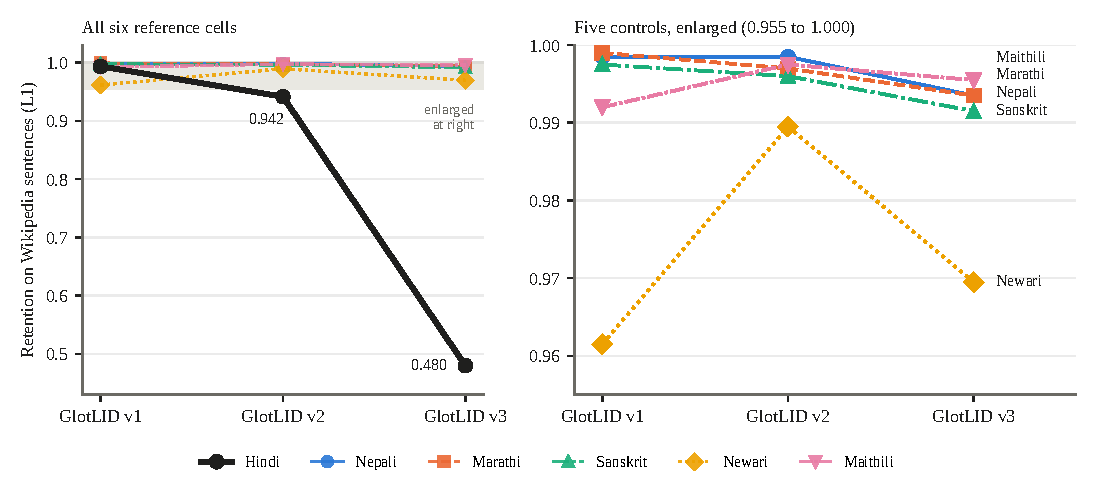
\includegraphics[width=\textwidth]{release_controls.pdf}
\caption{Retention on Panel 1 sentences across three GlotLID releases. The left panel shows all six cells on a common scale; the right panel enlarges the five controls, each with its own marker and line style and a direct label. Hindi changes much more than the controls, but the controls are not invariant: Newari varies from 0.962 to 0.990 and then 0.970. Exact counts and source-resampling intervals accompany the full results.}
\label{fig:controls}
\end{figure}

Hindi's change is much larger than those of the five controls, but the latter do not all remain within one percentage point (Figure~\ref{fig:controls}). Newari's L1 retention ranges from 0.962 to 0.990 across releases. The comparison shows selective deterioration on this Hindi cell, with useful within-panel controls. It does not establish a causal effect of adding Angika to the label inventory: training composition and other release changes were not held fixed.

The inventory itself can be read, and reading it narrows what the deterioration is about. Version 3 emits 302 labels that version 2 does not and drops 48 of version 2's, but 157 of the additions are \lab{und\_} placeholders for unseen Unicode categories rather than languages, leaving 145 genuine new classes. The removals include macrolanguage labels retired in favour of their members, \lab{ara\_Arab}, \lab{zho\_Hani} and \lab{nep\_Deva} among them, together with mergers such as the two Persian labels, relabelling such as Tagalog to Filipino, and individual labels that are no longer emitted. Seven of the genuine additions are Devanagari: Angika, Bodo, Dogri, Doteli, Goan Konkani, Kukna, and Sindhi written in Devanagari. Asking how much of each Panel~1 cell version 3 sends to any of those 145 separates the mechanism at issue from release changes in general, and the answer is concentrated. At one sentence the Hindi cell sends 0.5075 of its units to a label new in version 3. No other cell sends more than 0.0160: Newari 0.0160, Nepali 0.0050, Sanskrit 0.0045, Marathi 0.0040, Maithili 0.0010. The five controls are not merely stable in aggregate; the mechanism that moves Hindi barely reaches them.

It reaches them, though, and it reaches them in the same place. Of the 61 units those five cells send to a label new in version 3, 56 receive Angika---all nine of Sanskrit's, all thirty-two of Newari's, eight of Nepali's ten. Doteli, the new label nearest Nepali, takes two Nepali units in two thousand. So the Angika region draws from every Devanagari reference language in this panel and takes half of one of them. What distinguishes Hindi is the size of the pull rather than being the only language pulled on, which is the reading Section~\ref{sec:absorbing} returns to.

\subsection{Smaller inventories do not show the same Hindi loss}

The cross-instrument comparison gives a second description of the pattern. On the same Hindi sentence cell, \texttt{langid.py} and CLD3 retain 0.986 and 0.990. Neither carries any label in the protocol's Hindi-neighbourhood set. Their largest single non-Hindi destination receives only 0.008 of Hindi, so their lack of neighbourhood labels is not accompanied by a comparable relocation of the loss into Nepali, Marathi, or another available class.

This is an association between models with different inventories, not an experiment that removes labels from one fixed classifier. The distinction matters because fine coverage is also compatible with high Hindi retention: \lab{lid.176} retains every Hindi sentence in this cell, and GlotLID v1 retains 0.994 despite carrying six neighbourhood labels. OpenLID, with five such labels, retains 0.693 and assigns 0.256 of the Hindi cell to Awadhi. GlotLID v2 also carries Awadhi but assigns only 0.042 of the cell to it. Inventory availability identifies possible destinations; neither total label count nor neighbourhood count adequately describes the magnitude of loss in these comparisons.

\subsection{Retention and destination composition reveal different failures}\label{sec:transpose}

Hindi retention alone would favour several coarse identifiers. The transpose of the panel's routing table reveals a different problem. Among Hindi-labelled L1 units, the Hindi-sourced proportions are 0.626 for CLD3, 0.723 for \lab{lid.176}, and 0.828 for \texttt{langid.py}, compared with 0.978 for GlotLID v3. These proportions use the same panel mixture, with 2,000 units per source language, so they compare how the identifiers distribute a fixed evaluation collection.

\begin{figure}[tb]
\centering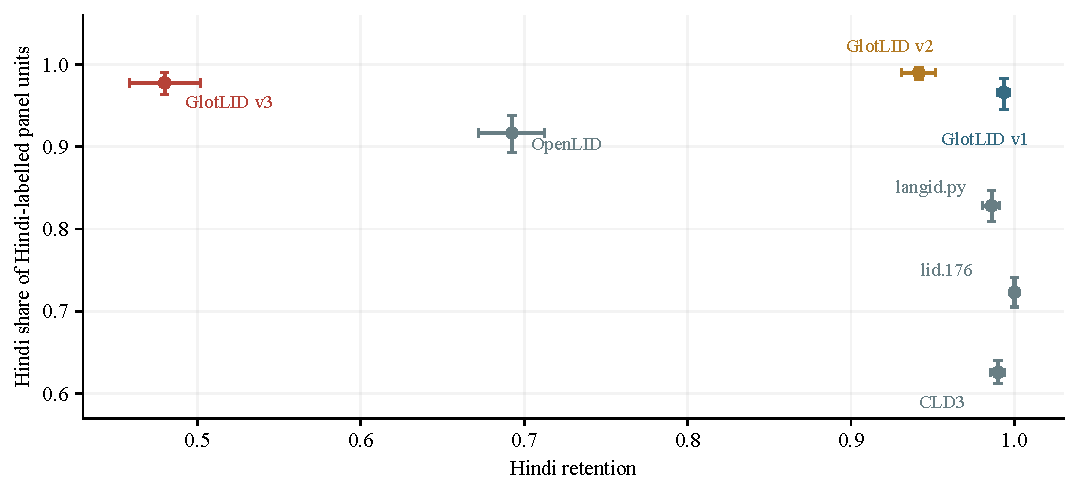
\includegraphics[width=\textwidth]{retention_composition.pdf}
\caption{Hindi retention and the Hindi-sourced share of Hindi-labelled Panel 1 sentences. Bars are 95\% source-resampling intervals, preserving the mixture's language weights. High retention and a clean destination bucket are different objectives. GlotLID v1 and v2 perform well on both axes here, so the contrasting coarse/v3 examples do not imply an unavoidable granularity-driven trade-off.}
\label{fig:transpose}
\end{figure}

The comparison is not a universal recall--precision law. GlotLID v2 retains 0.942 of Hindi and produces a Hindi bucket that is 0.990 Hindi-sourced on this mixture; v1 is also high on both measures (Figure~\ref{fig:transpose}). What the contrast establishes is that the model with a clean Hindi bucket can still lose much of the Hindi source material, while a model that retains Hindi can admit other source languages into that bucket. Neither statistic substitutes for the other.

\subsection{The absent source row, and what adding it does}\label{sec:seven}

Panel~1 has no Angika source row, and Angika is the label at issue. A destination-composition figure computed on a mixture that excludes the class in question is answering a narrower question than it appears to, so we report the seven-source variant. Regime~C supplies 2,000 marker-selected Angika Wikipedia sentences at the same cell size, drawn under the same minimum-length and script-purity filters, and we add them to the mixture as a seventh source row while leaving every other cell unchanged. Because the Angika cell is marker-selected, it favours Angika-distinctive writing and is not a representative Angika sample; it enters here as an additional source of units that a Hindi bucket might wrongly admit, which is a use its selection rule does not undermine.

The result is not a robustness check that leaves the picture intact. It reorders it (Table~\ref{tab:seven}). GlotLID v3's Hindi bucket moves from 0.978 to 0.976, a change of 0.002; every other identifier falls. \texttt{langid.py} falls furthest, by 0.341 from 0.828 to 0.487, and \lab{lid.176} ends lowest, at 0.427 from 0.723. The size of each fall broadly tracks how much of the Angika row the identifier sends to Hindi, and not how well it retains Hindi.

\begin{table}[tb]\centering\small\exhibit{seven_language}
\caption{Hindi retention and the Hindi-sourced share of the Hindi-labelled bucket on the six-language Panel 1 sentence mixture and on the same mixture with a seventh marker-selected Angika source row of equal size. Bracketed intervals are 95\% conditional source-resampling intervals preserving the designed cell weights; the OpenLID-v3 row is a later addition to the same mixture and is reported as point estimates. OpenLID-v3 carries no Newari label, which depresses both of its composition figures (Section~\ref{sec:modern}). The final column is the share of the Angika row each identifier assigns to Hindi. The Angika row is marker-selected and is not a representative Angika sample.}
\label{tab:seven}
\end{table}

The final column sorts the identifiers into three bands by where the Angika row goes, and the bands are what the table is for. Three identifiers send most of it to Hindi---\lab{lid.176} 0.958, \texttt{langid.py} 0.834 and CLD3 0.654---and give up between 0.183 and 0.341 of destination composition. For \texttt{langid.py} and CLD3 the reading is direct: neither carries any label in the protocol's Indo-Aryan neighbourhood, so Angika has nowhere else to go. \lab{lid.176} is different. Its inventory is sparse but includes Maithili and Bihari labels, and it still sends almost the whole row to Hindi, so label coverage does not by itself explain its placement. Four identifiers without an Angika label send the row mainly to neighbouring labels---GlotLID v1 0.111, OpenLID-v3 0.108, OpenLID 0.059, GlotLID v2 0.018---and give up between 0.018 and 0.094. Version 3 carries the Angika label, sends 0.001, and gives up 0.002. What separates the bands is the size of the fall, not its starting point: OpenLID-v3 begins low because it has no Newari label and the Newari row lands in its Hindi bucket (Section~\ref{sec:modern}), and it still falls only 0.057 when Angika is added.

Reading down the last two bands answers the question the table was built to ask. GlotLID v2 has no Angika class. On the seven-source mixture its Hindi bucket is 0.972 Hindi-sourced against v3's 0.976, a difference of 0.004 with intervals of [0.962, 0.981] and [0.961, 0.988] that overlap almost entirely; and it retains 0.942 of Hindi against v3's 0.480. The Angika class is not needed to keep other languages out of the Hindi bucket. Version 2's Awadhi, Bhojpuri, Magahi and Maithili labels had already done that, to within four thousandths. They take some Hindi too---v2 loses 117 of the 2,000 Hindi sentences, 83 of them to Awadhi---but a fraction of what v3 loses. Between the two releases, on this mixture, destination composition differs by four thousandths and Hindi retention by 0.462.

That is the finding, and it is sharper than a trade-off. A practitioner choosing between these two releases for Hindi is not weighing precision against recall: on this mixture the earlier release offers nearly the same precision with far higher retention. The comparison is about Hindi and about the cells measured here. Version 3 changes many other labels---302 additions, 145 of them genuine language classes, and 48 removals---and nothing in these experiments speaks to those other inventory changes; what they do show needs none of them, which is that a release evaluated only on the material its new classes name can regress badly on material they do not, and that this one did. The contemporary OpenLID-v3, which also carries no Angika class, retains 0.965 of the same Hindi. The precision and the loss are still two readings of one decision region, and Section~\ref{sec:absorbing} takes up its shape; on this comparison the region brings almost no precision that the earlier release lacked.

One smaller thing follows. The coarse/fine contrast of Section~\ref{sec:transpose} needs rereading: on the six-source mixture the coarse identifiers look merely imprecise, and on the seven-source mixture more than half of what each of their Hindi buckets contains comes from some other source language.

The coarse-model loss into Hindi also survives a lexical check on a weaker-provenance source row. A post hoc analysis derives Maithili-distinctive markers from held-out sentences excluded from the evaluation panel and restricts the panel to the 1,686 Maithili units carrying a marker. On those units, \lab{lid.176} retains 0.6845 and sends 0.6992 of its losses to Hindi. GlotLID v3 retains all of those selected units. The analogous Newari result differs: only 0.2607 of its marked-subset loss goes to Hindi, whereas about 0.725 goes to Marathi. The lexical restriction strengthens the evidence that the Maithili result is not explained solely by overtly Hindi-like material on the source wiki, but it does not make the selected subset an unbiased sample of Maithili writing. Both marked-subset results and their selection rules are in the accompanying repository.

\section{Hindi routing on reader-confirmed text}\label{sec:human}

\subsection{What was verified}

The reader judgments reused here were collected earlier, blind, for Hindi and Nepali text from six regimes: Wikipedia extracts, Wikipedia sentences, FLEURS read-speech transcripts \citep{conneau2022fleurs}, and IndicVoices read-speech, extempore, and conversational transcripts \citep{javed2024indicvoices}. This is text-language identification; no audio is classified. The stage-one sample contains 50 units per language/regime cell, drawn uniformly within each cell from a 7,767-unit analysis set at seed 20260903. Two readers judged a shuffled presentation that concealed the proposed language, domain, corpus, and identifier output. The options allowed Hindi, Nepali, mixed/code-switched, other language, and cannot tell; instructions prohibited machine assistance.

The panel was two readers, the second judging a 200-unit overlap; neither is an author of this paper. Both are adult secondary-school students in Simara, in the Nepal Terai, and both were compensated for the work. Their first language is Nepali and they read Hindi through the ordinary exposure of that belt---everyday interaction as much as media and entertainment---rather than through formal training; competence was established before the task by a panel interview and a sample reading, rather than assumed from residence or taken on self-report. Neither reads or understands Angika. The readers are not trained linguists and the design does not require them to be: the question put to them was which language a text reads as, not which of several closely related varieties a text belongs to.

The returned data bear this out. Reader 1's explicit language judgments agree with corpus provenance on 564 of 569 units, and the two readers agree with each other on 183 of 198 jointly answered items, as reported below. The second reader was there for that purpose, to put the first reader's identifications to an independent test, and they hold.

The response menu fixes what these judgments are about. It was built for a Hindi/Nepali separation task and offered no Angika option, so what a unit carries here is a positive identification as Hindi rather than a rejected Angika reading. That is the quantity the paper uses. Material removed from the Hindi label is lost to Hindi whatever another label's claim on it turns out to be, so text identified as Hindi by a reader who saw it blind is sufficient for every claim made below; ruling an Angika reading in or out is a different study, requiring Angika readers and an Angika option.

Reader 1 answered 593 of 600 units: 569 received an explicit Hindi or Nepali judgment, 20 were mixed/code-switched, and four were uncertain. Seven were blank. Of the 569 explicit language judgments, 564 matched corpus provenance (99.1\%). Reader 2 answered a separately shuffled 200-unit overlap; the readers agreed on 183 of 198 jointly answered items (92.4\%). A literal \lab{n} entry is retained as a disagreement. These are raw agreement proportions, not chance-corrected reliability scores. The earlier design's rule for expanding annotation was not triggered; no additional annotation is collected here.

Before running the comparison, we link each returned judgment to its original text and recorded hash. None of the 600 normalized texts exactly matches a unit in the later reference panels. The checked texts therefore form a separate evaluation set; their verification rate cannot be transferred to those panels.

Our primary analysis uses the 564 units for which reader 1 confirms the provenance label. We then check the 179 units confirmed by both readers and, separately, score predictions against all 569 explicit reader-1 language judgments. Mixed, uncertain, and blank responses are excluded from single-language scoring but remain in the records. These stratified subsets describe the verified texts, and their pooled proportions are descriptive of those texts rather than estimates of language-wide or web-wide prevalence.

\subsection{Hindi-identified text can still leave the Hindi label}

Table~\ref{tab:human} compares the hash-verified GlotLID releases on the same confirmed units. GlotLID v1 retains 278 of 279 Hindi units and v2 retains 267. Version 3 retains 216, while 59 receive Angika. The Nepali control is more stable: v1 and v2 each retain 284 of 285 confirmed units, and v3 retains 279. The historical v3 top labels reproduce exactly on all 600 sampled units under its native prediction path.

\begin{table}[tb]\centering\small\exhibit{human_summary}
\caption{Retention on the existing blinded verification sample. The primary subset requires reader 1 to confirm provenance; the stricter subset requires both readers. Counts and proportions are descriptive within these selected subsets.}\label{tab:human}
\end{table}

The two-reader Hindi subset retains the same qualitative failure: v1 and v2 each retain all 86 units, whereas v3 retains 76 and sends nine to Angika. Against all explicit reader-1 language judgments, including those that disagree with provenance, v3 retains 216 of 280 Hindi-labelled units and v1 retains 279. The conclusion is therefore not created by excluding the five provenance disagreements, although neither subset is a representative Hindi corpus. Restating the claim these counts support: v3 assigns Angika to 59 units that a blind reader called Hindi, of which v1 assigned 58 to Hindi and v2 assigned 52. Nine of the 59 were called Hindi by both readers independently, and both earlier releases assigned all nine to Hindi.

Source differences are visible within the checked sample. Version 3 retains 18 of 46 confirmed Hindi Wikipedia sentences, 27 of 41 Wikipedia extracts, and 45 of 50 conversational transcripts. The other transcript cells remain separate in Appendix~\ref{app:human}. The small cell sizes preclude a broad register ranking. The Nepali IndicVoices material was collected in India, so its language verification does not establish Nepal provenance or representativeness of Nepali varieties.

Two short examples illustrate the discrepancy. Both readers judged \dev{खेडिया झल्लो खैर, अलीगढ़, उत्तर प्रदेश स्थित एक गाँव है।} (``Khediya Jhallo is a village in Khair, Aligarh, Uttar Pradesh'') and \dev{फिर, लक्खा सिंह ने भजन गायकी की कमान संभाली.} (``Then Lakkha Singh took over the bhajan singing'') as Hindi. Version 3 assigns Angika to both; v1 and v2 assignments are retained in the example records. These are the lowest-ID qualifying short examples in the Wikipedia-extract and FLEURS regimes, respectively, selected for explanation after scoring. They are not additional independent observations, and the English glosses are explanatory rather than human verification data.
\section{What the loss depends on, and what it does not}\label{sec:source}

The Hindi source-by-length profile is a separate experiment from the artifact/control length comparison in Section~\ref{sec:lengthaudit}. Here the reference language remains Hindi and we compare Wikipedia, news, and curated ILI sources. Each source is reported separately. The Wikipedia and news collections differ in domain, register, and collection process together, so the comparison does not isolate any one of them; Section~\ref{sec:overlap} removes training overlap from that list for the Wikipedia side by measuring it directly.

\begin{figure}[tb]
\centering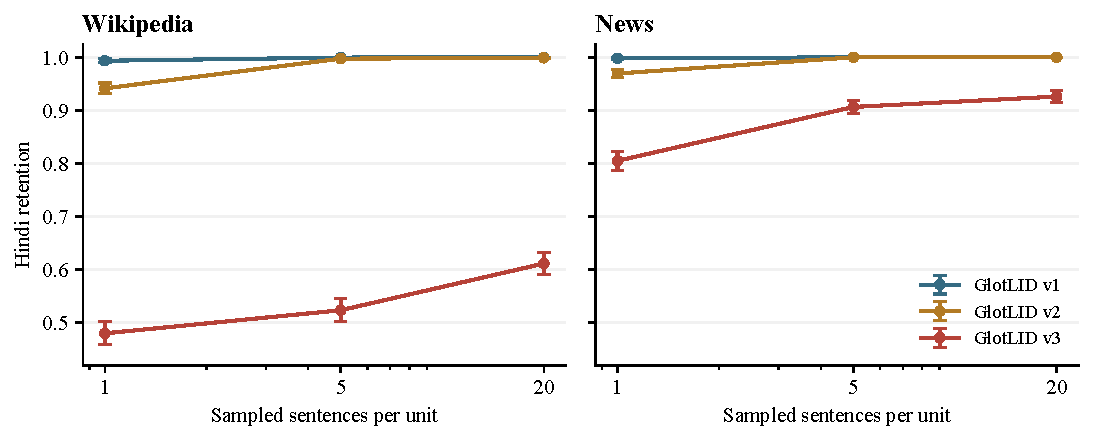
\includegraphics[width=\textwidth]{source_length.pdf}
\caption{Hindi retention by source and unit length. L5 and L20 aggregate sampled sentences from one source, not complete documents. Error bars are 95\% conditional source-resampling intervals. Identifiers share the same input units within each cell. Different length cells may use different eligible source subsets; the profiles are descriptive, not estimates of an intervention that lengthens identical documents.}
\label{fig:source}
\end{figure}

GlotLID v3 retains 0.805 of Hindi news sentences, compared with 0.480 of Wikipedia sentences. Its source-resampling intervals are [0.787, 0.822] and [0.458, 0.502], respectively. On five sampled sentences, the retentions are 0.907 and 0.524; on twenty, 0.926 and 0.612 (Figure~\ref{fig:source}). Longer news units therefore show much less loss than news sentences, while a substantial loss remains on the twenty-sentence Wikipedia cell. The experiment does not justify summarizing the model's Hindi behaviour with one unqualified error rate.

The destination of news loss remains concentrated. Of the 390 Hindi news sentences that v3 assigns elsewhere, 364 receive Angika: 0.933 of the loss, or 0.182 of the full Hindi news cell. The broader neighbourhood receives 0.977 of the loss. All 187 losses at L5 and all 148 at L20 receive Angika. The magnitude varies with source and length even where the main destination is stable.

ILI provides an additional provenance regime, not a domain-matched replication of the web audit. On its filtered Hindi train and development cells, v3 retains 0.867 and 0.862; the test cell, whose original Hindi material is partly social media, yields 0.954. We report these descriptive values with their separate source compositions. The earlier GlotLID releases generally retain more Hindi in these cells as well, although their losses are not uniformly negligible: v2 retains about 0.921 on ILI Hindi train and 0.924 on development.

\subsection{Holding sources fixed across nested units}

The initial profiles use different eligible samples at different lengths. To test whether source selection alone produces their pattern, we reconstruct the original 2,000 Hindi L20 sources in each collection and build nested first-one, first-five, and first-twenty sampled-sentence units. Every reconstructed L20 text matches its stored counterpart exactly. Applying the original minimum-token and script-purity filters jointly at all three lengths retains 1,760 Wikipedia and 1,334 news sources. The shorter units cause the exclusions; none is selected by a model prediction. All three lengths now use identical sources and common inclusion rules.

\begin{figure}[tb]\centering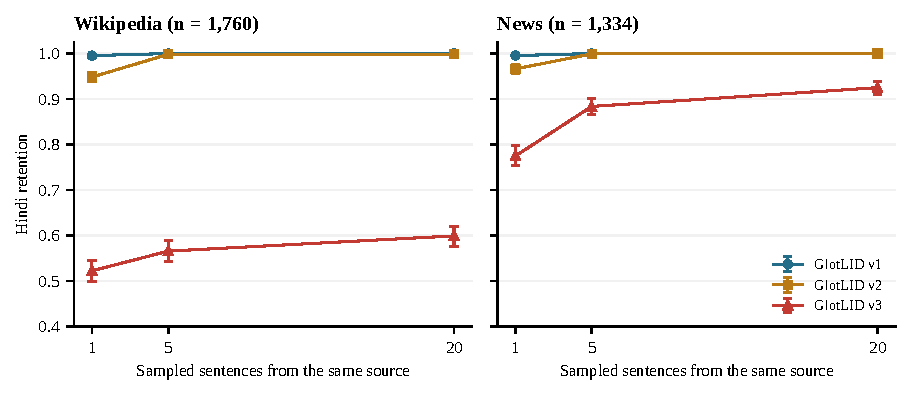
\includegraphics[width=\linewidth]{nested_retention.pdf}
\caption{Hindi retention on nested sampled-source units. Each source contributes all three lengths. Intervals pair source resampling across lengths within each model; the unit remains an aggregate of sampled sentences, not a verified consecutive passage.}\label{fig:nested}
\end{figure}

On the fixed Wikipedia source set, v3 retains 920 of 1{,}760 units at L1 (0.523), 996 at L5 (0.566), and 1{,}055 at L20 (0.599); Figure~\ref{fig:nested} shows all three lengths together. The paired increase from L1 to L20 is 0.077, with a 95\% source-resampling interval of [0.048, 0.105].

The increase is larger on news. Of 1,334 units at each length, v3 retains 1,034 at L1 (0.775), 1,179 at L5 (0.884), and 1,234 at L20 (0.925). The paired increase is 0.150 [0.127, 0.172]. Every observed L20 loss in both collections goes to Angika. Versions 1 and 2 retain nearly all L20 Hindi on these same source sets (Appendix~\ref{app:nested}).

The source contrast therefore survives fixing the eligible documents across lengths. Extending the input changes its lexical content as well as its length; the comparison does not isolate token count from additional evidence. It concerns the sources that survive the joint filters, and Wikipedia and news remain different collections.

\subsection{Sensitivity to source concentration}

The original Hindi L1 samples contain 1,871 Wikipedia and 1,954 news source clusters, with at most four selected sentences in any cluster. Giving each observed source cluster equal weight changes v3 retention from 0.480 to 0.473 for Wikipedia, and from 0.805 to 0.806 for news. Removing the largest cluster gives 0.480 and 0.805 after rounding. The four longer original cells each have one selected unit per recovered source cluster; all six cells contain no exact text duplicates. These checks show that a heavily repeated article does not drive the measured contrast. They do not remove publisher-level dependence, near-duplicates, or training overlap. Full per-release sensitivities are supplied in Appendix~\ref{app:nested} and the machine-readable records.
\subsection{Prior exposure to the evaluated text does not account for the loss}\label{sec:overlap}

The Hindi cells are drawn from Leipzig Wikipedia, and Wikipedia is among the sources of the identifier's own published training collection, so some evaluated sentences may have been seen during training. That overlap can be measured. The released GlotLID v3.1 collection distributes one Hindi Wikipedia file of 233{,}956{,}634 bytes and 999{,}281 non-empty lines \citep{glotlid-corpus-v31}. Matching the Panel 1 Hindi L1 units against it by exact text after Unicode normalization and whitespace collapse, 1{,}554 of 2{,}000 units are present and 446 are not.

Retention divides accordingly. GlotLID v3 retains 743 of the 1{,}554 present units, a fraction of 0.478, and 217 of the 446 absent units, 0.487. These are the two parts of the 960 units retained overall. Destinations divide the same way: 789 present and 226 absent units receive the Angika label, fractions of 0.508 and 0.507, together the 1{,}015 Angika assignments reported above. At five sentences the corresponding retentions are 0.516 and 0.526.

The intervals here use the same conditional source-cluster resampling as the rest of the sampled-panel analysis, giving [0.452, 0.503] for the present group and [0.441, 0.533] for the absent group. Clustering makes almost no difference to this particular comparison, for a reason specific to it: the Hindi L1 cell's 2,000 units fall in 1,871 recovered source clusters, and only 40 of those clusters contain both a present and an absent unit, so the split is very nearly between clusters rather than within them. Resampling clusters also lets us report the quantity the two separate intervals could not, namely the present-minus-absent difference, which is $-0.008$ with interval [$-0.063$, $0.043$]: from 6.3 percentage points lower to 4.3 points higher retention for units present in the file. This is an observed association between presence in the published file and retention, not an estimate of a causal exposure effect, and it is small against the 0.325 Wikipedia--news gap that an exposure account would have to explain.

We compared the two groups' own properties before reading those rates, because the division is not random: it is the intersection of two Leipzig draws from the same source, and retention here responds to unit length (Section~\ref{sec:source}). Their median token counts are 16 and 17 and their mean Devanagari shares 0.9988 and 0.9980, so the groups are alike on the properties this design measures.

The match test is exact, so it misses paraphrase, retokenization, and light editing between the two draws; some units counted as absent are present in the collection in a form the test does not detect. If those missed matches are unrelated to routing, the misclassification attenuates any difference toward zero; if they are related, the direction of the bias is unknown. Either way this null is weaker evidence than a positive difference would have been. What it supports is that prior exposure to the evaluated sentences does not account for the Wikipedia loss under this test. Because presence in the file shows no association with retention within the Wikipedia cell, exposure is also a weak candidate for the Wikipedia--news contrast, although we did not measure the news cell's membership in the same collection. The released collection is an edited version of the training data rather than the training data itself, so the measurement concerns the published artifact.

\subsection{Register does not account for the source contrast}\label{sec:register}

Calling the Wikipedia--news difference a difference of source leaves the operative word unanalysed, and the literature on small Wikipedia editions supplies a specific candidate for what it might stand for (Section~\ref{sec:related} above). Small-edition Wikipedia text is disproportionately formulaic stub material: high in proper-noun density, thin in the function-word evidence a character- or token-feature classifier can use. Both of the illustrative sentences in Section~\ref{sec:human} are of that kind, one a geographic stub and one a name-heavy singer sentence. If the account is right, the Wikipedia cell should be the name-dense, function-word-poor cell, retention should fall as function-word evidence thins, and matching the two cells on that evidence should close much of the gap. The account is testable on the units we already hold, so we test it.

Three instruments, none of them fitted to the retention outcome. The first is function-word evidence, counted with the 25-token Hindi list fixed for the Angika marker derivation before this analysis and used here unchanged. The second is a rare-token rate, the share of a unit's tokens absent from the ten thousand most frequent types of the identifier's own published Hindi training file, where proper nouns and place names concentrate. The third is a stub-template match: whether a unit's final token trigram is among the two hundred most frequent sentence-final trigrams of held-out Hindi Wikipedia, held out by excluding every source cluster represented in the evaluation panel. Matching strips edge punctuation from tokens and markers alike, because the Wikipedia cell ends 91.6\% of its units with a danda and the news cell ends 69.9\% of its units with a full stop, and seven of the 25 stored markers carry an attached danda; without that normalization the instrument credits Wikipedia with evidence the news cell cannot register.

The cells are close on all three, and the small differences do not run the way the account requires (Table~\ref{tab:register}). Function-word rate is 0.111 on Wikipedia against 0.104 on news, and the share of units containing no function-word match at all is 0.112 against 0.153: the losing cell has marginally more of this evidence, not less. Rare-token rate is 0.114 against 0.127, again favouring the losing cell, and here the comparison is conservative in the other direction as well, since the reference vocabulary is itself Wikipedia-derived. Only the stub-template share separates the cells as predicted, 0.172 against 0.117, and it does not predict retention: template-matching Wikipedia units retain 0.453 against 0.486 for the rest, a difference of $-0.032$ with source-clustered interval [$-0.091$, $0.027$], and in the news cell template units retain 0.803 against 0.805.

The decomposition settles it. Reweighting the news cell to the Wikipedia cell's distribution of any of these observables, and of token count, leaves news retention at 0.803 to 0.811 against its unadjusted 0.805, absorbing between $-1.8\%$ and $0.6\%$ of the 0.325 gap; no interval reaches $2\%$, so the intervals exclude any large share. Within the news cell retention does rise with function-word count, from 0.732 at none to 0.877 at four or more. Within the Wikipedia cell it does not rise steadily, running 0.491, 0.415, 0.506, 0.485, 0.608 across the same buckets; only the top bucket, whose units average 29 tokens against 14 to 22 in the others, stands clearly higher. Whatever separates these two collections is not on this axis in the losing one.

\begin{table}[tb]\centering\small\exhibit{register}
\caption{Register composition of the two Hindi L1 cells and the share of their retention gap absorbed by reweighting the news cell to the Wikipedia cell's distribution of each observable. Bracketed intervals resample source clusters within each cell.}
\label{tab:register}
\end{table}

The instruments are coarse---a 25-token list is a thin proxy for function-word evidence, a final-trigram match a thin proxy for stub structure---so the null bounds these operationalizations rather than register in general. Within that bound it removes the most available reading of the source contrast: the Wikipedia loss is not a stub artifact.

\subsection{Proximity to the absorbing class's training material accounts for part of it}\label{sec:ngram}

One instrument does better, and it is the model's own. The Angika class was trained on a single Wikipedia-derived file (Section~\ref{sec:trainingclass}), so if that class carries Hindi material the material is Wikipedia-register Hindi, and the region learned around it would sit nearer Wikipedia-style Hindi than news Hindi. GlotLID is a fastText classifier and represents text as a bag of character n-grams, so the natural measure is n-gram proximity to the two published training files. We score each Hindi unit by its mean log-probability per character trigram through pentagram under add-one smoothed models estimated from the published Angika file and from a size-matched sample of the published Hindi file, and report the Angika-minus-Hindi difference.

This instrument behaves as the account predicts, and it is the only one that does. Hindi Wikipedia units sit nearer the Angika file than Hindi news units by 0.121 in mean score. Within each cell, proximity predicts routing: retention falls from 0.560 to 0.370 across Wikipedia proximity deciles and from 0.875 to 0.695 across news deciles, and in both cells the units routed to Angika sit nearer the Angika file than the units retained, by 0.048 on Wikipedia and 0.078 on news. That within-cell gap is not a length effect. The routed units are the shorter ones, at a median of 13 tokens against 20 on Wikipedia and 14 against 16 on news, but longer units score nearer the Angika file rather than further, so standardizing each cell to its own token-length distribution widens the gap rather than closing it, to 0.054 and 0.088 with intervals of [0.032, 0.077] and [0.061, 0.114]. It is positive in all ten token bands, and within every band retention still falls as proximity to the Angika file rises.

What the instrument does not do is carry the source contrast. Reweighting the news cell to the Wikipedia cell's distribution of n-gram proximity moves news retention from 0.805 to 0.769, absorbing 0.112 of the 0.325 gap with an interval of [0.070, 0.159]. About a ninth, where the register instruments absorbed nothing.

Appendix~\ref{app:register} records all four instruments and their parameters. So ``domain'' in Section~\ref{sec:source} is no longer entirely unanalysed, and it is not yet analysed either. Proximity to the Angika class's training material is a real component of the Wikipedia loss and a small one; eight ninths of the contrast between the two collections remains unaccounted for by anything measured here.

\section{Confidence does not recover source retention}\label{sec:confidence}

\subsection{A substantial share of demonstrated errors survives every allowed confidence threshold}

FineWeb-2 defines a per-language confidence threshold from the label's score distribution $X$, clipped to $[0.3,0.9]$ \citep{penedo2025fineweb2}:
\begin{equation}
\tau=\max\{0.3,\min\{0.9,\operatorname{Med}(X)-\sigma(X)\}\}.
\end{equation}
Write $S(\tau)$ for the share of a scored collection with the same assigned label whose scores are at least $\tau$. Since $S$ is non-increasing and the rule clips $\tau$ to $[0.3,0.9]$, every allowed threshold satisfies $S(0.9)\leq S(\tau)\leq S(0.3)$. A score below 0.3 cannot pass this rule; a score of at least 0.9 passes every permitted threshold; a score between the bounds requires the actual threshold to determine survival.

We score the original 4,000 Hindi Panel 1 units through GlotLID v3's own ranked prediction path. Every top label matches the stored panel prediction. Of the 1,015 L1 units assigned to Angika, 574 score at least 0.9: a fraction of 0.566, with source-resampling interval [0.535, 0.596]. At L5, 277 of 952 such units clear 0.9, a fraction of 0.291 with interval [0.263, 0.320]. These are lower bounds on the fractions that would pass any threshold allowed by the stated confidence rule, conditional on the evaluated model and panel inputs.

\begin{figure}[tb]
\centering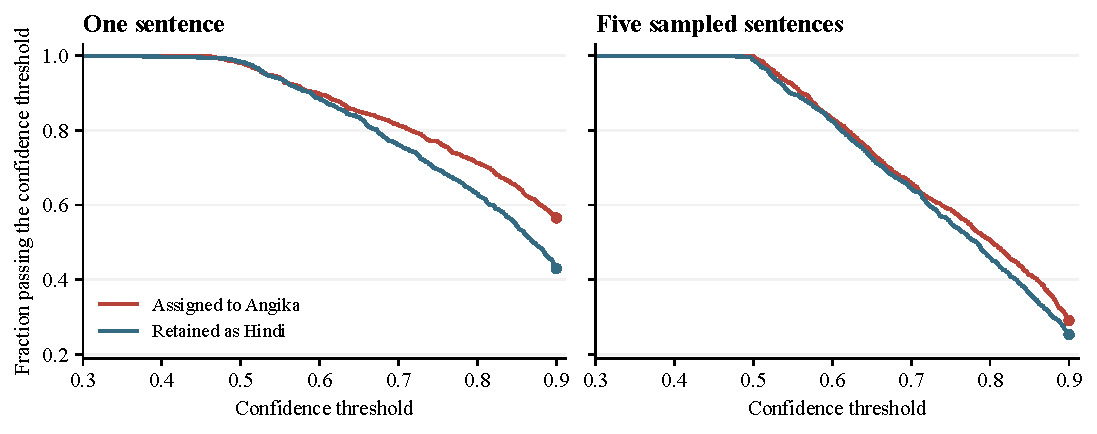
\includegraphics[width=\textwidth]{confidence_survival.pdf}
\caption{Observed confidence-survival functions for Hindi Panel 1 units, grouped by the label received. Curves show the fraction scoring at least each threshold; the right endpoints give survival under the largest permitted threshold. Survival through this confidence rule does not imply survival through subsequent filters or demonstrate that these panel units entered the released corpus.}
\label{fig:confidence}
\end{figure}

None of the scored Hindi units falls below 0.3, which establishes survival at the lowest threshold and not at every threshold; the units between the bounds depend on a label-specific production score distribution we do not estimate. What Figure~\ref{fig:confidence} shows is the part that does not depend on it: raising the threshold to its maximum still leaves more than half of these errors in place.

The wrong assignments are also not restricted to low scores. At L1, the median score for Hindi units assigned to Angika is 0.925, versus 0.871 for those retained as Hindi. Their source-resampling median intervals are [0.914, 0.935] and [0.857, 0.886]. A softmax score is not a calibrated probability of correctness; what makes it the relevant quantity here is that it is the score to which the corpus pipeline applies its filtering rule. Results for both lengths are in Appendix~\ref{app:confidence}.

\section{A contemporary comparison: OpenLID-v3}\label{sec:modern}

The official OpenLID-v3 release provides a current comparison alongside the historical models \citep{fedorova-etal-2026-openlid,hpltopenlidv3model}. Its inspected binary emits 195 labels including the non-language class. It carries Hindi, Nepali, Maithili, and Awadhi, but not Angika, Newari, or Braj. We evaluate common newline-to-space input and OpenLID-v3's published recommended normalization separately, using top-1 routing without a confidence cutoff. The recommended example's additional 0.5 cutoff would introduce abstention and is not silently included in these retention rates.

On Panel 1 Hindi sentences, OpenLID-v3 retains 0.965 under common preprocessing and 0.957 under recommended preprocessing. Both exceed the historical 201-label OpenLID artifact's retention of 0.693 and GlotLID v3's 0.480. On the full six-language mixture, the Hindi-sourced shares of its Hindi-labelled buckets are 0.740 and 0.754, respectively.

Those destination figures also reflect a coverage limitation: OpenLID-v3 has no Newari label, so the Newari row has nowhere to go and lands largely in Hindi. When the unsupported Newari source row is excluded, precision is 0.993 under common preprocessing and 0.994 under recommended preprocessing. Removing a source row changes the evaluation mixture, so these figures answer a different question from the six-language estimates.

On the 279 reader-confirmed Hindi units, the contemporary model retains 271 under common preprocessing and 266 under recommended preprocessing, against GlotLID v3's 216; on the 86 units confirmed by both readers it retains 85 in either condition. It retains 284 of 285 Nepali units under common preprocessing and all 285 under recommended. Its nested Wikipedia and news L20 retention exceeds 0.998 in both preprocessing conditions (Appendix~\ref{app:nested}). Thus the severe v3 Hindi loss does not generalize to every contemporary identifier. Model choice remains relevant, and retaining Hindi well does not by itself establish a precise Hindi destination on a mixture containing unsupported languages. Appendix~\ref{app:modern} records the binary's identity, its coverage, and both preprocessing conditions in full.

\section{Released partitions as routing diagnostics}\label{sec:artifacts}

\subsection{The Angika-labelled split and its controls}\label{sec:angikasplit}

We examine the complete \lab{anp\_Deva} training shard: 57,997 documents, read at the frozen repository revision and SHA-256 recorded in Appendix~\ref{app:repro}. Two GlotLID releases assign 0.991 and 0.982 of these documents to Hindi. These are assignment rates under the specified auditing binaries; no Hindi-content estimate is inferred.

\begin{table}[tb]
\centering\small
\exhibit{angika_audit}
\caption{Shares assigned to Hindi in the Angika-labelled released split and marker-selected Angika controls. The split contains 57,997 whole documents; controls contain 868 selected articles and 3,269 selected sentences. Whole-article controls were measured for v1 and v2 from hash-verified binaries. The columns specify units, not matched length distributions.}
\label{tab:angika}
\end{table}

GlotLID v1 and v2 assign Hindi to 0.109 and 0.020 of the selected Angika control sentences. Neither carries an Angika label: their contribution is to distinguish the selected controls behaviourally from the released split, not to recognize Angika correctly as a class. Their whole-article control rates are 0.083 and 0.010, compared with 0.991 and 0.982 on the split (Table~\ref{tab:angika}).

The control articles are selected from 1,028 Angika Wikipedia extracts. An article enters when at least half of its eligible sentences carry an Angika marker under the previously fixed tagger; the sentence control consists of the 3,269 stored Angika-marked sentences. The markers were derived by contrasting token frequencies with Hindi reference text. They provide a lexical distinction independent of the evaluated classifiers, but favour Angika-distinctive writing. They do not make Wikipedia a domain-matched control for crawled web documents.

The same tagger also partitions the extract instead of selecting from it, which gives a reading of the whole population rather than of its selected part alone. Of the extract's 4{,}823 filtered sentences, 3{,}269 carry Angika-distinctive markers, 1{,}158 carry Hindi-distinctive markers, and 396 carry neither. GlotLID v3 assigns Hindi to 0.0009, 0.2599 and 0.3232 of the three groups and to 0.0896 of the extract as a whole, and it assigns Angika to 0.7375 of the Hindi-marked group (Table~\ref{tab:groups}).

The lexical split is not an artifact of the tagger that produced it. Identifiers carrying no Angika label have no reason to treat the two marked groups differently, yet v1 and v2 separate them by factors of nine and forty-six in Hindi routing, assigning the Hindi-marked group to Hindi at 0.995 and 0.936, while sending the Angika-marked group to Magahi, Bhojpuri, Awadhi and Maithili. The extract is therefore a mixture rather than homogeneous Angika: its Hindi-marked quarter carries Hindi-distinctive vocabulary and is assigned to Hindi by binaries that carry no Angika label, whatever its origin on the wiki.

\begin{table}[tb]\centering\small\exhibit{angika_groups}
\caption{The 1,028-article Angika Wikipedia extract partitioned by the fixed lexical tagger, with the share of each group that GlotLID v1 and v3 assign to Hindi and to Angika. Version 1 carries no Angika label, so its Angika column is empty by construction; its separation of the first two groups shows that the lexical split is not an artifact of the tagger. Version 2's rates to Hindi on the three groups are 0.020, 0.936 and 0.667.}
\label{tab:groups}
\end{table}

The marker selection also limits what the Angika recognition check establishes. GlotLID v3 assigns the Angika label to 0.9911 of the marked sentence collection and Hindi to 0.0009. Thus the model recognizes this selected Angika material while also assigning substantial Hindi material to Angika. Recognition on these controls is compatible with contamination or other defects in training data; it does not identify or exclude those explanations. Section~\ref{sec:trainingclass} reads the label's published training collection directly and finds elevated Hindi assignment within it, which bears on the first explanation without isolating it.

\subsection{Length explains part of the reading, but not the observed sentence contrast}\label{sec:lengthaudit}

The split's documents and the Angika articles differ greatly in length. Their medians are 1,640 and 257 characters. Comparing their aggregate document assignment rates alone therefore leaves a clear alternative explanation. We address it with a length characterization over the same populations and a deterministic sentence draw.

For each arm, common support is the intersection of the populations' empirical 5th--95th percentile character-length ranges. We begin with six equal-width bins on log length and use a deterministic merging rule until retained bins meet the minimum of 50 units and 30 source documents from each population. Exact boundaries, merging rules, coverage, and counts accompany the analysis. We retain both the sentence arm and the document arm, regardless of how much support each provides.

At sentence level, all six bins remain. Common support is 32--177 characters, covering 85.8\% of the selected Angika sentences and 90.8\% of the 50,000 sampled split sentences. GlotLID v1 assigns a larger fraction of split sentences to Hindi in every bin, with differences of 0.827--0.892. For v2 the differences range from 0.741 to 0.936 (Figure~\ref{fig:lengthaudit}). Each difference is measured against the same model's Angika control at comparable character lengths. The intervals resample source articles within each population and bin, conditional on the fixed support and boundaries. They are pointwise sensitivity intervals, not simultaneous evidence of separation at every possible length.

\begin{figure}[tb]
\centering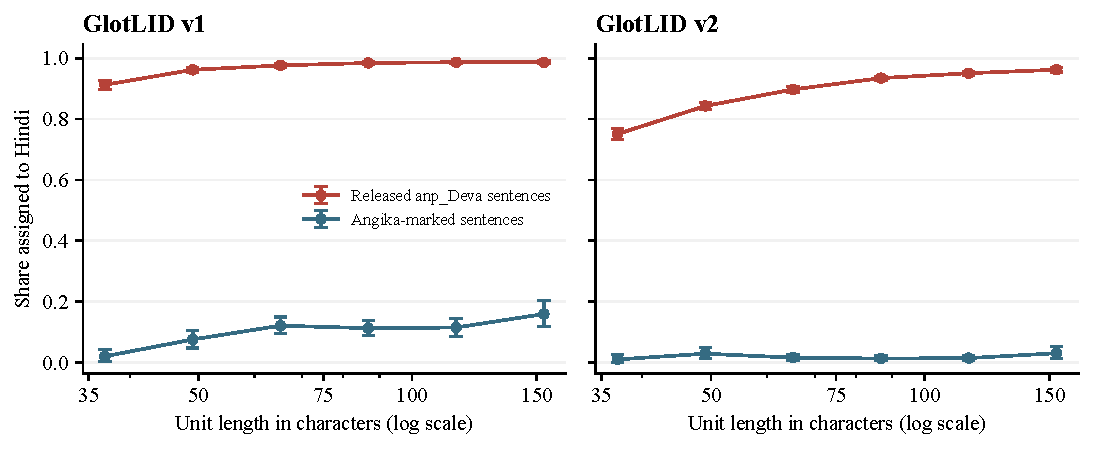
\includegraphics[width=\textwidth]{angika_length.pdf}
\caption{Hindi assignments across the common sentence-length region. Each point is a bin mean positioned at the geometric midpoint; lines connect descriptive bin summaries and are not fitted curves. Bars are pointwise 95\% conditional source-resampling intervals. Populations remain marker-selected Angika Wikipedia sentences and sentences sampled from the released split. Comparable length does not make their domains or selection mechanisms comparable.}
\label{fig:lengthaudit}
\end{figure}

The document arm supports a much weaker resolution. Its common region is 561--1,114 characters, and the fixed occupancy rule merges the initial six bins into one. That interval includes 104 Angika articles and 11,497 split documents, only 12.0\% and 19.8\% of the respective populations. Within it, v1's Hindi assignment rates are 0.163 on the control and 0.987 on the split; v2's are 0.010 and 0.978. The differences are large, but a single supported interval is not a document-length response curve.

Length alone does not account for the large sentence-level contrast on the measured common support. It remains an open alternative outside that support: the design covers neither the complete document-length range nor the domain difference between Angika Wikipedia and a crawled web artifact, and no independently curated Angika web control was available.

\subsection{The published training collection for the absorbing label}\label{sec:trainingclass}

The label that absorbs the Hindi loss has a published training collection, and it can be read with the same binaries. In GlotLID v3.1 the Angika directory holds a single file of 1{,}232{,}680 bytes drawn from Wikipedia \citep{glotlid-corpus-v31}; the fixed segmenter and the panel filters leave 3{,}970 sentences.

GlotLID v1 and v2 assign Hindi to 0.252 and 0.176 of those sentences. The informative comparison is with the same binaries' rates on the marker-selected Angika control sentences, 0.109 and 0.020, which the same binaries reproduce exactly before the collection is read. Both models therefore assign Hindi to the training collection several times more often than to the selected Angika control. GlotLID v3 is not used here, because the collection is its own published training material.

The collection is not the control corpus under a different name: 0.286 of its filtered sentences match a sentence of the 1{,}028-article Angika extract by exact text. Under a one-sided rule that looks only for Angika markers, 0.786 of the collection's filtered sentences carry one, against 0.674 of the extract's 4{,}823 (3{,}251 sentences); the two-sided tagger that defines the controls, which also weighs Hindi markers, labels 3{,}269 of the extract's sentences Angika-marked (0.678). The released collection thus carries a higher share of Angika-marked sentences than the wiki text it derives from, which is consistent with the dataset card's description of it as an edited version.

Two limits determine what this shows. The card describes v3.1 as the data used to train GlotLID v3 with some edits, so it is a derivative, and how a rate measured on it relates to the corresponding rate on the material the model was trained on is unknown: the card records that edits were made, not their direction or their effect on these rates. And an assignment rate is not a content estimate (Section~\ref{sec:design}). What these readings establish is a behavioural contrast, not the collection's linguistic composition.

\subsection{Awadhi is a contrasting second case}\label{sec:awadhi}

We next read the complete \lab{awa\_Deva} training shard at the same frozen repository revision. It contains 1,902 documents. OpenLID and GlotLID v1 and v2 all carry Awadhi labels and reproduce their archived predictions on the ILI Awadhi controls exactly. We use these three models for the new comparison. The coarse identifiers lacking an Awadhi label cannot validate recognition of that label, and GlotLID v3 is not used as an adjudicator of this artifact. The earlier releases are themselves related models; no family member supplies independent linguistic ground truth.

All three models assign most of the shipped documents to Awadhi: 0.865 for OpenLID, 0.746 for GlotLID v1, and 0.955 for v2. Their Hindi assignments are 0.093, 0.236, and 0.025, respectively (Table~\ref{tab:awadhi}). At sentence level the models assign more material to other labels, but their Hindi assignment rates remain far below the Angika split's corresponding GlotLID readings. The sentence analysis draws 50,000 unique eligible sentences from a pool of 55,736, using the fixed segmenter and seed.

\begin{table}[tb]
\centering\small
\exhibit{awadhi_audit}
\caption{Assignments on the released Awadhi-labelled split. Each model is reported separately; Hindi and Awadhi shares need not sum to one because other labels are possible. Document figures enumerate the entire training shard. Sentence figures describe the fixed 50,000-sentence draw after segmentation and filtering.}
\label{tab:awadhi}
\end{table}

The ILI controls show why each model and source division needs its own comparison. On ILI Awadhi test sentences, OpenLID, v1, and v2 retain 0.730, 0.683, and 0.801 as Awadhi. Retention is lower on train and development. The test results therefore cannot stand in for all curated Awadhi; Appendix~\ref{app:awadhi} reports the three divisions separately.

The sentence-length comparisons retain six descriptive bins for each ILI division. Their common support covers roughly 86--89\% of the reference units and 88--90\% of the released-split sentence draw. For all three identifiers, the split's Hindi assignment rate is lower than the ILI training reference's rate in every retained bin. Comparisons with development and test vary by model and bin, and are reported without document-resampling intervals because ILI's parent-document identities are unavailable.

The Awadhi audit establishes a contrasting identifier profile on another heavily filtered labelled split: the Angika pattern does not replicate here. It certifies nothing about Awadhi purity either, since the models disagree materially and curated literary sentences are not a domain-matched web reference. These two cases support targeted artifact audits, not a prevalence estimate for language mislabelling across the corpus.

One difference between the two cases is structural rather than linguistic. The auditing models here---OpenLID, v1 and v2---all carry an Awadhi label, so they can route Awadhi material to Awadhi. The same models carry no Angika label, so when they read the Angika-labelled split they must route its contents somewhere else, and Hindi is the nearest available destination. A reading in which a label-less model sends Angika-labelled documents to Hindi is therefore close to uninformative on its own.

The control is what makes the Angika reading informative. The same label-less binaries, reading marker-selected Angika Wikipedia, assign Hindi to 0.109 and 0.020 of it: lacking an Angika label does not by itself drive this material to Hindi. The split reads at 0.991 and 0.982 against those controls, and the separation holds in every shared sentence-length bin (Section~\ref{sec:lengthaudit}). The comparison is thus within model and against a reference sharing the model's coverage limitation, which the aggregate document rate alone would not have given. The Awadhi case tests whether the pattern recurs on another heavily filtered split; it is not a matched control for the Angika case.

\subsection{Removal fractions do not identify what survived}\label{sec:removal}

The released retained and removed files provide a separate observable: how much of each labelled partition remains after the relevant filtering stages. We read the exact document counts from Parquet metadata, summing every training shard at a single frozen repository revision. The dataset card specifies that the retained-plus-removed data are the collection after global deduplication \citep{fineweb2-dataset}; the released pipeline configuration records the stage order but not the production checkpoints \citep{finewebpipeline}. Consequently, these fractions describe removal from that released post-deduplication partition, not loss from the original crawl or a measurement of global deduplication itself.

\begin{table}[tb]
\centering\small
\exhibit{removal_counts}
\caption{Complete retained and removed training-shard counts at the frozen FineWeb-2 revision. Fractions are removed divided by retained plus removed. File-byte fractions use stored Parquet sizes, including compression and metadata; they are not fractions of uncompressed linguistic text. Neither fraction isolates a particular filter.}
\label{tab:removal}
\end{table}

For Angika and Awadhi labels, the document-removal fractions are 0.9995 and 0.9986. Hindi's is 0.4372 (Table~\ref{tab:removal}). The corresponding file-byte fractions differ, including 0.3850 for Hindi, illustrating why a file-size ratio should not silently be used as a document ratio. These counts are a census of the published files, so no sampling interval is attached.

The two audited labels have similarly extreme removal fractions, yet their retained documents receive contrasting model readings. Thus the size of a removal fraction cannot certify the linguistic quality of the remainder. It also cannot identify which filter acted: quality rules, repetition checks, confidence decisions represented in the release, and language-specific filtering need stage-specific provenance to disentangle. Whether the Angika label received the particular wordlist precision filter, whose high-affinity word lists follow \citet{bapna2022building}, is not established by this audit. The fractions measure operations on labelled partitions, not the availability or fate of the corresponding languages.

\section{The Angika label as an absorbing class}\label{sec:absorbing}

The preceding sections measure the Angika label from several directions. Gathered by what they say about one decision region, they support a single reading, set out here with the alternatives it does not exclude.

A misplaced boundary between two confusable classes would typically leak in both directions: some Angika called Hindi, some Hindi called Angika, with the errors concentrated where the model is least certain. That is a common pattern rather than a requirement, so the five observations below are read as departures from it rather than as proof against every boundary account. The Angika--Hindi relationship in version 3 departs from it on each.

\textbf{The exchange is one-way.} Because the tagger partitions the whole Angika extract rather than selecting from it, the asymmetry can be stated without a selected denominator (Section~\ref{sec:angikasplit}, Table~\ref{tab:groups}). Version 3 sends 0.0896 of that extract to Hindi, and 0.0009 of its Angika-marked part. Against 0.5075 of Hindi Wikipedia sentences and 0.182 of Hindi news sentences crossing the other way, the ratio is about six to one on the whole extract and about five hundred and fifty to one on the marker-selected control alone. The asymmetry holds under every denominator; its magnitude does not, and the range is what the evidence supports.

The extract's Hindi-marked quarter is the reason the unselected figure understates the contrast, and counting version 3 wrong on it would invert the error: that quarter carries Hindi-distinctive vocabulary, and two binaries carrying no Angika label call it Hindi better than nine times in ten. The same table reads the other way too. Version 3 assigns 0.7375 of exactly that material to Angika---text carrying Hindi-distinctive vocabulary, in a population wholly separate from Panel 1. The absorption is not confined to the Hindi panels.

\textbf{The absorbed material is not near a boundary.} Among Hindi Panel~1 sentences the median confidence of units assigned to Angika is 0.925, against 0.871 for units retained as Hindi (Section~\ref{sec:confidence}), and the source-resampling intervals [0.914, 0.935] and [0.857, 0.886] do not overlap. A top-1 score alone would not settle this, since a softmax over 2{,}102 classes distributes mass by how crowded a label's neighbourhood is, and Angika's may be less crowded than Hindi's. The ranked path settles it. For the 1{,}015 Hindi sentences routed to Angika the runner-up is Hindi in 93.6\% of cases, so the model is choosing between exactly the two labels at issue; but the runner-up's median score is 0.069, it never exceeds 0.4944, and the median top-1-minus-top-2 margin is 0.853, with 77.6\% of these units above a margin of 0.5. Hindi is the second choice and a distant one. The model is more confident when it takes Hindi away than when it keeps it, and it is not hesitating. This is why more than half of these errors survive every threshold the published confidence rule permits: they are not marginal cases, and no threshold that rule permits will reach them. At five sentences the margin narrows to a median of 0.610 and Hindi is runner-up in 99.9\% of cases---the same pattern with more Hindi evidence in the input.

\textbf{The absorbed material does not resemble Angika.} On the dimensions that separate the two classes in their own published training data, the Angika class's training file, segmented and filtered into its 3{,}970 sentences, has a Hindi function-word rate of 0.019, with 81.8\% of those sentences carrying no Hindi function-word match at all, and a rare-token rate of 0.399 against the Hindi vocabulary; the marker-selected control is more extreme still, at 0.001, 98.2\% and 0.437. The Hindi sentences version 3 routes into Angika sit at 0.122 and 0.101---squarely among the Hindi material, and slightly further from the Angika profile than the Hindi sentences it retains. Whatever the Angika region responds to, it is not lexical similarity, on this measure, to the text the label was trained to name.

The lexical instrument is licensed for this comparison and not for others: a Hindi-distinctive word list can compare populations, which is what is done here, but cannot establish that routed text is more Hindi than retained text, which is why Section~\ref{sec:register} reads only its reweighting result as a test. Routed units carry a higher function-word \emph{rate} than retained units, 0.122 against 0.100, but a lower \emph{count}, 1.76 against 2.04, because they are shorter, at a median of 13 tokens against 20; Section~\ref{sec:register}'s buckets are counts, which is why retention does not rise steadily across them. Nothing here supports the stronger claim that version 3 preferentially removes the sentences carrying the most Hindi evidence. By count it removes those carrying slightly less.

Section~\ref{sec:ngram} put the same question to character n-grams and got the opposite sign. There the routed units sit nearer the Angika file than the retained ones, by 0.048 on Wikipedia and 0.078 on news, and nearer still once unit length is held fixed. The two instruments disagree, and which of them the model follows is the finding rather than a difficulty. A word list is what separates these languages for a reader; a character n-gram model is closer to what a fastText classifier computes over, and the region tracks that one. Which representation an identifier separates languages by is a live design question rather than a settled one \citep{meister-etal-2026-language}. The representation is not the culprit, though. Version 2 is the same architecture over the same kind of features, and its Awadhi, Bhojpuri, Magahi and Maithili labels hold this material out of the Hindi bucket while losing 0.0585 of the Hindi cell, against v3's 0.520. What an n-gram space accounts for is how a region can be drawn where a reader would not draw one. It does not account for why this class and not its neighbours. With that bound in place, the disagreement is describing one region: not a boundary drawn in the wrong place between two vocabularies, but a region drawn in a space where that vocabulary is not what is being compared, which is why the absorbed text can read as Hindi to someone who knows Hindi and sit inside an Angika decision region at the same time.

\textbf{The region is active on both sides at once.} It takes 0.9911 of marker-selected Angika and 0.5075 of Hindi Wikipedia, and sends 0.001 of the Angika row to Hindi (Section~\ref{sec:seven}). A boundary that had failed in one direction would not typically also hold this firmly in the other. The exclusion, though, is not the region's achievement: GlotLID v2's neighbouring labels keep the same material out of Hindi at 0.018, with no Angika class and a Hindi loss of 0.0585 rather than 0.520. What is peculiar to version 3 is not that Angika stays out of Hindi. It is that Hindi comes in.

\textbf{The draw does not look like a general cost of finer resolution.} Version 3 adds seven Devanagari classes and one of them takes almost everything that moves. Of the 61 units the five non-Hindi Panel~1 cells send to any class new in the release, 56 receive Angika: all nine of Sanskrit's, all thirty-two of Newari's, eight of Nepali's ten (Section~\ref{sec:routing}). The remaining five are three Marathi units to Goan Konkani and two Nepali units to Doteli---the new class nearest Nepali, taking two units in two thousand---while Bodo, Dogri, Kukna and Sindhi in Devanagari receive none at all. The languages Angika draws from are not ones a boundary with Angika would be drawn between: Newari is Tibeto-Burman and Sanskrit is Old Indo-Aryan, and version 3 sends material from both to a class for an Eastern Indo-Aryan lect. A reader who took the Hindi loss for the ordinary price of a finer inventory would expect the other six new classes to be collecting too. They are not. This is one region's reach rather than a property of the resolution.

These five together support reading the Angika label in this release as an absorbing class: a decision region containing Angika and a large, confidently held portion of Hindi. How such a region arises is a further question, and Section~\ref{sec:trainingclass} bears on it, reporting that GlotLID v1 and v2 assign Hindi to 0.252 and 0.176 of the label's own published training collection against 0.109 and 0.020 on the marker-selected control---several times the control rate, under binaries that cannot express the Angika label. Contamination of the training class by Hindi material would produce both that reading and a region of this shape.

It is not the only thing that would. The elevated Hindi assignment is measured on an edited derivative of the training data, so its magnitude in the material version 3 actually saw is unknown. A region of this shape could equally arise from label weighting that gives the smaller class disproportionate influence, from feature-extraction settings that leave the two classes poorly separated in the represented space, or from either in combination with contamination, and the evidence here does not rank them. Nor does it establish that the same region existed in whichever binary made historical corpus-production decisions. Separating these calls for controlled retraining that varies the label setup and the training material independently, which Section~\ref{sec:release} sets out. What these measurements do establish is the shape of the region in the released artifact, and that a region of this shape is consistent with both of the release's headline behaviours at once.

\section{Discussion: what a language label measures}

\subsection{What destination inspection leaves out}

The findings point to a practical problem: inspecting a language-labelled collection cannot tell us how much material from that language was sent elsewhere. Equation~\ref{eq:identity} is not a new estimator, but much audit practice proceeds as though the destination count settled the question. Even when the destination is precise, $B_j$ determines neither the original supply $N_j$ nor the retained fraction $T_{m,c}(j,j)$.

The distinction has a large practical consequence in the measured v3 configuration. Its Hindi bucket is 97.8\% Hindi-sourced on the designed sentence mixture, yet only 48.0\% of the source Hindi reaches that bucket. The separate reader-confirmed sample shows that Hindi-to-Angika routing also occurs on text people identify as Hindi. Holding sources fixed preserves the contrast between the Wikipedia and news length profiles. A routing profile measured on one source or release therefore gives an incomplete account of another.

For corpus construction, this means that a precise language label can conceal a substantial change in the available source material. Whether that change affects a downstream model depends on later filtering, data mixing, and training. Those effects are a motivation for examining routing, rather than a result measured here.

\subsection{How to audit the selection process}

An informative audit needs both sides of the routing decision. Independently labelled source samples show what stays under its language label and where the rest goes. Destination evaluation then shows what arrives from other languages, either on a declared evaluation mixture or through annotation of the actual collection. Finally, testing the applied filtering rule shows which observed errors it can remove. Confidence, agreement between models, and removal counts (Section~\ref{sec:removal}) each answer only part of this question.

When specialist annotation is unavailable, comparisons against reference controls can identify a corpus partition that warrants investigation. They cannot establish its linguistic composition by consensus; annotation of the partition itself can, and where it has been organized at scale it has found labelled cells that are largely another language \citep{vanstrien2025fineweb}. The Angika and Awadhi case studies illustrate this role: the Angika split/control contrast persists over the available shared sentence lengths, whereas Awadhi gives a different profile despite similarly severe removal. These findings help direct an audit without estimating the prevalence of mislabelling across FineWeb-2.

\subsection{What would settle the release difference}\label{sec:release}

Section~\ref{sec:absorbing} argues for the shape of the decision region and lists the accounts of its origin that the present evidence cannot rank. What would separate them is controlled retraining, and the obvious shortcut does not work. Removing Angika from the outputs of an already trained classifier only forces another prediction; it does not isolate the effect of having included Angika during training. The informative experiment holds the texts, feature-extraction settings, and training procedure fixed while varying the label setup, and then separately holds the label setup fixed while varying the training material of the class under test---in particular, while removing from the Angika class the material that reads as Hindi under binaries that cannot express the Angika label.

The source contrast needs its own experiment, and a better hypothesis than the one Section~\ref{sec:register} rules out. Wikipedia and news may differ in how well their vocabulary and recurring expressions are represented in the training data, and differences in source balance or training weights could then contribute to the larger Wikipedia loss. A useful test would hold the label inventory fixed and vary source composition or weighting, evaluating each model on the same untouched Wikipedia and news sets. What we can say from the present data is narrow: the contrast is not exposure to the evaluated sentences (Section~\ref{sec:overlap}), not function-word evidence, name density, stub structure, or unit length at fixed unit type (Section~\ref{sec:register}), and it survives holding the eligible documents fixed across nested lengths. Proximity to the Angika class's published training material accounts for about a ninth of it (Section~\ref{sec:ngram}), which is the only positive component measured and points at the training material rather than at the two collections.

Whether other classes behave this way is a third question, and Section~\ref{sec:routing} answers it only within Devanagari, where the answer is negative. Testing it elsewhere would not require reference corpora for the 145 classes version 3 adds. It would require them for the donors---the established languages a new class might draw from---which are by construction the better-resourced side of each pair. Donors can be identified before any such corpus is built, by the reading Section~\ref{sec:trainingclass} already makes for Angika: run a binary that cannot express the new class over that class's own published training collection, and record which label receives the material. Ranking the 145 that way, of which 109 are Latin-script, eleven Cyrillic, seven Devanagari and five Arabic, would yield a short donor list, and provenance-labelled cells for those donors under the filters of Section~\ref{sec:design} would support the same retention and destination measurements reported here. Because that collection is an edited derivative, the ranking selects what to measure and is not itself evidence about routing.

Production history is a separate uncertainty. A present-day binary hash matching the evaluated v3 does not establish which binary was used for every historical crawl. These limits leave the routing failure intact while keeping its explanation open.

\section{Limitations}

The reference panels cover selected Devanagari languages and sources. Their larger cells use provenance labels rather than unit-level human annotation. The separate human-checked sample contains Hindi and Nepali only, uses a limited reader overlap, and excludes mixed, uncertain, and unanswered units from single-language scoring. Its response menu offered no Angika option, so it establishes identification as Hindi and not the absence of an Angika reading. It does not validate Angika or Awadhi corpus composition or establish population-wide error rates. The Angika controls are marker-selected Wikipedia text, not representative Angika web material, and the seventh source row of Section~\ref{sec:seven} inherits that selection; their document-length common support remains narrow. The one-way exchange ratio of Section~\ref{sec:absorbing} ranges from about five hundred and fifty to one on that selected control to about six to one on the unselected extract, and the extract is itself a mixture containing Hindi-marked material, so neither endpoint is a clean estimate of the asymmetry between the two languages.

The nested units hold sources fixed but concatenate sampled sentences, not reconstructed continuous passages. Source bootstrap intervals condition on the observed samples and do not address annotation error, publisher dependence, or domain transfer. Training overlap is measured separately for the Hindi Wikipedia cell in Section~\ref{sec:overlap}, by an exact-match test that may attenuate a true difference and is not applied to the other cells. ILI lacks parent-document identities, and the exact-duplicate and source-concentration checks bound rather than certify the independence of the texts.

The register analysis of Section~\ref{sec:register} uses three coarse instruments---a 25-token function-word list, a frequency-based rare-token rate, and a final-trigram template match---and its null result bounds those operationalizations rather than register in general. Its n-gram proximity measure uses unigram models over character n-grams estimated from published files, which is an approximation to a supervised classifier's representation and not that representation; the 0.112 it absorbs, and the length-standardized within-cell gap reported with it, are properties of that approximation.

The published GlotLID v3.1 collection is an edited derivative of the training data rather than the training data itself, so the rates of Section~\ref{sec:trainingclass} describe the published collection, and their relation to the rates on the material the model was trained on is unknown. The absorbing-class reading of Section~\ref{sec:absorbing} is an interpretation of the released artifact's behaviour, not a measurement of its training data or its parameters, and the alternatives listed there remain open. Model comparisons change training and coverage together; no causal inventory effect is identified. OpenLID-v3's two preprocessing conditions are reported separately, not used to tune a best-performing recipe. The exact FineWeb-2 production snapshot remains unestablished. Confidence survival concerns the evaluated binary and one rule, not inclusion after all pipeline filters. There is no downstream model-training experiment.

\section{Conclusion}

A precise Hindi-labelled bucket can conceal substantial loss of Hindi source material. The measured GlotLID v3 configuration demonstrates the gap, and blind reader judgments place it on text people call Hindi. No account of it that we could measure removes it: prior exposure to the evaluated sentences, register and name density, unit length at fixed unit type and with sources held fixed, and every confidence threshold the published rule permits. Only proximity to the absorbing class's own training material accounts for any part of the Wikipedia--news contrast, and for about a ninth of it. OpenLID-v3's stronger retention shows that severe loss of this size is not shared by every contemporary identifier.

The two headline numbers are two readings of one decision region, and measuring both sides of it changes what the release looks like. On a designed mixture of six 2,000-unit Wikipedia cells plus a seventh of 2,000 marker-selected Angika sentences, identifiers that route the Angika row to Hindi fall as far as 0.427 destination composition, while the three GlotLID releases and the 201-label OpenLID, which route it to neighbouring labels or to Angika, hold above 0.85 whether or not they name Angika; OpenLID-v3, which routes it to neighbours but has no Newari label, moves from 0.740 to 0.683. On that same mixture the immediately preceding release reaches 0.972 against v3's 0.976, and retains 0.942 of Hindi against 0.480. Destination composition is always a property of the mixture it is computed on, and a different mixture would move these figures; what they show on this one is that the release with the new class is four thousandths more precise than its predecessor and retains 46 percentage points less of the Hindi source.

A new fine-grained label is not simply an improvement in resolution to be evaluated on the material it names. It is a change to the extent of every neighbouring class, and in this release measurably so: the new class draws units from all five of the other Devanagari reference languages, two of which are not closely related modern varieties of Angika. Evaluated only on Angika, this class is a success, recognizing 0.991 of marker-selected Angika. Evaluated on both sides of the decision it makes, it is where half of a large language's Wikipedia text goes instead of its own label. Both measurements were always available; only one of them is usually taken.

Corpus audits should therefore examine both what reaches a language label and what is sent elsewhere, then test which errors survive the relevant filters. Released partitions and comparisons between identifiers can help locate problems, but establishing their true language composition requires separate evidence. Measuring routing in this way makes the selection of training material visible without assuming its cause or its downstream effect.

\section*{Ethics}
The reader judgments reused here come from two adult participants who were compensated for their time and who judged a shuffled presentation blind to the proposed language, the source corpus, and every identifier output. No new human annotation was collected for this study. The evaluated texts are public corpora and released corpus partitions, used under their original terms and identified by release, revision, and checksum; no personal data was collected and no attempt was made to identify the author of any evaluated text. The study measures released artifacts on public material; it deploys no system and alters no corpus. Specific model releases and corpus partitions are named so that the measurements can be checked and repeated, and the results characterize those artifacts under the stated conditions rather than the practices of the groups that produced them.

\section*{Disclosure}
The author's company, Swar Nepal Pvt.\ Ltd., develops language-data resources for Nepali, one of the reference languages. Nepali enters this study only as a control: it is a reference language whose retention is reported for comparison with Hindi's. The Hindi findings do not depend on the Nepali cells. Removing them would change some reported counts---the control units sent to Angika would fall from 56 of 61 to 48 of 51---but not the Hindi results. Existing reader judgments are reused with their original blinding and recorded disagreements; no new human annotations were collected for this study. Claude (Anthropic) and ChatGPT (OpenAI) were used as AI assistants for programming and drafting; the author checked all analyses and results and takes responsibility for the content.

\section*{Data and code availability}
Code, unit identifiers, text hashes, per-unit predictions (including the per-unit OpenLID-v3 predictions), reader judgments linked to their units, source clusters, marker lists, results, protocols and provenance records are available at
\begin{center}\url{https://github.com/oliromin/instrument-paper}\end{center}
Third-party corpora are not redistributed: they are identified by release, revision and checksum, and a script rebuilds every evaluated text from them and checks it against its stored hash. Model binaries are identified by checksum and are not included. From the named inputs the repository regenerates every table and figure and checks every reported number. Code is released under the MIT License and data under CC BY 4.0.

\bibliographystyle{compling_url}
\bibliography{references}
\clearpage\appendix
\renewcommand{\thesection}{\Alph{section}}
\renewcommand{\theHsection}{appendix.\Alph{section}}
\FloatBarrier
\section{Panel 1 retention}\label{app:panel1}

Table~\ref{tab:panel1} reports the initial two lengths with their actual denominators. A dash indicates that the model cannot emit an accepted label for the source language. It denotes unsupported coverage, rather than an observed success rate. Source-resampling intervals for every supported cell, and paired release differences, are provided in the machine-readable results. Cells with zero observed errors may have a degenerate resampling distribution; this does not establish zero future error.

\begin{table}[htbp]
\centering\small\setlength{\tabcolsep}{4pt}
\exhibit{panel1_retention}
\caption{Retention on Panel 1. Rates are rounded from exact counts to three decimal places using a consistent half-up convention. Apparent values of 1.000 can therefore include a small nonzero loss; exact counts accompany the table in the repository.}
\label{tab:panel1}
\end{table}

At L1 the six language cells have equal size. L5 uses the complete eligible pool for Marathi, Sanskrit, Newari, and Maithili, whose cells are smaller than 2,000. The destination-composition analysis preserves these observed mixture weights at each length. The initial panel and its later extension are not pooled.

\FloatBarrier
\section{The second panel and length extension}\label{app:panel2}

Table~\ref{tab:panel2} retains source regimes and ILI divisions. Regime C's Angika units are selected using the marker criterion; the longer cells include most eligible source units. LD denotes a whole Angika article in that regime's construction and is distinct from the 868-article selection used in the artifact/control audit. The small L20 cells---31 Angika, 59 Marathi, 278 Sanskrit, 119 Newari, and 21 Maithili units---remain descriptive and do not evaluate the earlier protocol's size-dependent thresholds. Full results for the coarse identifiers are in the accompanying prediction-derived tables.

\begin{table}[htbp]
\centering\small\setlength{\tabcolsep}{4pt}
\exhibit{panel2_retention}
\caption{Per-language retention in Panel 2 and the separate Wikipedia L20 extension. Dashes denote unavailable label coverage. The ILI test cells retain their original split identity after filtering.}
\label{tab:panel2}
\end{table}

\FloatBarrier
\section{Paired Hindi contrasts and confidence}\label{app:confidence}

The intervals below describe the original Hindi profiles. Within each cell, the bootstrap resamples the same sources jointly across model releases, preserving their paired predictions. It does not treat the releases as independent studies. These original profiles use potentially different eligible source subsets at different lengths; their intervals therefore do not estimate a paired length effect. The later nested-source comparison holds sources fixed and is reported separately in Section~\ref{sec:source} and Appendix~\ref{app:nested}. Table~\ref{tab:hindiresponse} reports the profiles.

\begin{table}[htbp]
\centering\footnotesize\setlength{\tabcolsep}{3pt}
\exhibit{hindi_release_contrasts}
\caption{Hindi retention and paired release differences. Bracketed intervals are conditional 95\% source-resampling intervals. Each row holds 2,000 units.}
\label{tab:hindiresponse}
\end{table}

The confidence table separates assignments to Angika from retention as Hindi, with each group using its own denominator. Scores exceeding one by approximately $10^{-5}$ are a recorded numerical feature of the native fastText output and do not affect the 0.9 comparison. The interpretation uses score inequalities, not probability calibration. The 574 and 277 Angika-assigned units above the ceiling are observed counts; confidence-stage survival does not establish inclusion in a published corpus. Table~\ref{tab:confidencefull} gives both lengths.

\begin{table}[htbp]
\centering\small\setlength{\tabcolsep}{4pt}
\exhibit{confidence_scores}
\caption{GlotLID v3 confidence on the fixed Hindi panel units. The share column uses the group size $n$ as denominator. None of the 4,000 scored units falls below 0.3.}
\label{tab:confidencefull}
\end{table}

\FloatBarrier
\section{Length comparison and Awadhi reference controls}\label{app:awadhi}

The Angika common-support rule uses linear empirical quantiles and six initial logarithmic bins. All bins include their lower edge and exclude their upper edge, except that the final bin includes both. A deficient bin has fewer than 50 units or 30 source documents from either population. We repeatedly merge the leftmost deficient bin leftward if its ordinal midpoint lies in the lower half of the current bin sequence, and rightward otherwise; endpoint bins merge inward and ties go left. This deterministic rule yields six sentence bins and one document bin. The displayed boundaries are rounded for reading; computations use the unrounded stored edges. Table~\ref{tab:angikabins} reports the retained bins.

\begin{table}[htbp]
\centering\footnotesize\setlength{\tabcolsep}{3pt}
\exhibit{angika_length_bins}
\caption{Angika-reference versus released-split Hindi assignment rates. $A$ denotes the marker-selected reference and $S$ the released split. The gap is $q_S-q_A$. Intervals are pointwise conditional source-resampling sensitivities. The document interval fails the three-bin resolution criterion and is not presented as a curve.}
\label{tab:angikabins}
\end{table}

For the Awadhi sentence comparison, the common-support edges are determined separately for ILI train, development, and test. All three retain six bins by unit occupancy. Parent-source identities are known on the released-split side but unavailable for ILI, so cluster sufficiency and clustered intervals cannot be established for that reference side. Binwise assignment tables for every model and ILI division are included in the machine-readable results; the absence of source identities is explicitly recorded there. These descriptive profiles neither pool ILI divisions nor infer the language composition of the released artifact. Table~\ref{tab:awadhicontrols} reports the reference controls.

\begin{table}[htbp]
\centering\small
\exhibit{awadhi_controls}
\caption{Awadhi reference controls, with original ILI divisions preserved. The same verified binaries reproduce all archived labels on these units. Rates concern the filtered panel cells, not the entire unfiltered shared-task corpus.}
\label{tab:awadhicontrols}
\end{table}

The original unfiltered ILI test evaluation is also in the repository. None of the seven identifiers covers all five task labels. A macro F1 can be defined on a fixed reference label set even when a classifier cannot emit a class, but that score would combine coverage failure with discrimination under a different task setup. We therefore report output coverage and per-language retention rather than use such a score as directly comparable with the shared task's 0.958.

\FloatBarrier
\section{Recorded protocol outcomes}\label{app:protocols}

Each analysis this paper reports is listed here with the status defined in Section~\ref{sec:uncertainty} and, where it was specified to look for something, with the direction it was given and the outcome.

Pre-specified before their runs: the Panel 1 and Panel 2 draws and filters, the three-release retention comparison, the cross-instrument comparison, the source-by-length profiles, the nested-source construction, the source-concentration checks, the confidence-survival counts, and the contemporary comparison of Section~\ref{sec:modern}.

Hypothesis-informed, with procedures recorded before the computations they govern: the length characterization of Section~\ref{sec:lengthaudit} and the Awadhi comparison of Section~\ref{sec:awadhi}. In both, the bin rules, occupancy minima and merging order were fixed before any binwise assignment rate was inspected.

Post hoc: the Angika reference audit, the released-split reading, the Maithili and Newari marked-subset restrictions of Section~\ref{sec:routing}, the label-inventory comparison, and the three analyses below.

The label-inventory comparison of Section~\ref{sec:routing} reads both releases' emitted label lists from the hash-verified binaries, separates the \lab{und\_} placeholders from genuine language classes before any routing outcome is inspected, and was specified to look for a second Panel~1 cell losing a substantial share of its units to a class new in version 3. None was found; the largest non-Hindi share is Newari's 0.0160 against Hindi's 0.5075, and the result is reported as a null. That the other cells' small losses share Hindi's destination was not predicted and is reported as an observation.

The seven-source destination composition of Section~\ref{sec:seven} fixed the seventh cell's identity and size before any composition was recomputed. It carried no directional prediction; the reported quantity is the change in each identifier's destination composition when the Angika row is added.

The register analysis of Section~\ref{sec:register} was specified to look for three things: a Wikipedia cell lower in function-word evidence and higher in name density than the news cell, retention rising with function-word evidence within each cell, and reweighting absorbing a substantial share of the source gap. None of the three held. The shares absorbed, between $-0.018$ and $0.006$ with no interval reaching $0.02$, are reported as a null, and the source contrast is left unexplained rather than reattributed.

The n-gram proximity analysis of Section~\ref{sec:ngram} was specified to look for the same three things on its own instrument. The first two held and the third held in part: reweighting absorbed 0.112 of the gap against an expectation of a substantial share, and it is reported as a partial account. Its length standardization is a further post hoc check, prompted by the observation that units routed to Angika are shorter than units retained, and specified to look for the within-cell gap disappearing once token length was held fixed. It did not disappear; the standardized gap is slightly larger than the raw one, and that is how both are reported.

\FloatBarrier
\section{Register instruments and the seventh source row}\label{app:register}

The function-word instrument of Section~\ref{sec:register} is the 25-token Hindi-distinctive list of the Angika marker instrument: \dev{इन}, \dev{इसके}, \dev{इस}, \dev{इसमें}, \dev{इसी}, \dev{कर}, \dev{गया}, \dev{दो}, \dev{इसकी}, \dev{उसे}, \dev{थी}, \dev{जा}, \dev{उन्होंने}, \dev{थे}, \dev{लिए}, \dev{जाती}, \dev{हैं}, \dev{है}, \dev{सकता}, \dev{वे}, \dev{करने}, \dev{किया}, \dev{उस}, \dev{था}, shown after the edge-punctuation stripping described there, which merges two stored entries and leaves 24 distinct types. The list was derived by contrasting token frequencies with Angika reference text and is Hindi-distinctive by construction; its association with retention is therefore not evidence for anything, and only the reweighting result is read as a test.

The rare-token instrument counts a unit's tokens absent from the 10,000 most frequent types of the published GlotLID v3.1 Hindi file, which contains 999,281 non-empty lines and 546,551 distinct types under the same tokenization. The vocabulary size was fixed before any retention outcome was computed. The template instrument uses the 200 most frequent final token trigrams of 262,659 held-out Hindi Wikipedia sentences, held out by excluding every source cluster represented in the evaluation panel.

The reweighting in Table~\ref{tab:register} places each cell's units in buckets of the relevant observable---function-word counts of zero through four or more, six token-count bands, template match, and five rare-token bands---and recomputes the news cell's retention under the Wikipedia cell's bucket weights. An observable that accounted for the source contrast would drive the residual gap toward zero. All four leave it between 0.323 and 0.331 against a raw gap of 0.325.

The n-gram instrument of Section~\ref{sec:ngram} uses character trigrams through pentagrams with a leading and trailing space, add-one smoothing over the union vocabulary of the two reference files, and a Hindi reference size-matched to the Angika file by character count under reservoir sampling at seed 20260912; the two files contribute 196{,}708 and 239{,}536 n-gram types over a union of 351{,}270. Its reweighting uses eight equal-width buckets spanning the pooled score range, and its interval comes from 1{,}999 replicates at the same seed, resampling source clusters in both cells; the 2{,}000 news units fall in 1{,}954 recovered source clusters. The register reweightings use the same replicate count and seed. The length standardization of the within-cell routed-versus-retained gap uses five token bands---ten or fewer, eleven to fourteen, fifteen to nineteen, twenty to twenty-nine, and thirty or more---weighted by each cell's own band occupancy, with ten routed and ten retained units required for a band to contribute; its intervals come from 1{,}999 replicates at the same seed, resampling source clusters in the same way. Regressing the score on routing status and log token count gives coefficients on routing of 0.054 and 0.086 in the two cells, against standardized gaps of 0.054 and 0.088.

The seventh source row of Section~\ref{sec:seven} is the Regime C Angika L1 cell, 2,000 units drawn at seed 20260908 from a filtered pool of 3,315 marker-selected sentences, falling across 796 source articles, which supply the resampling clusters for that row.

Three counts of Angika Wikipedia appear in this paper and they are not the same quantity. The artifact audit of Section~\ref{sec:artifacts} uses the 1,028-article extract, whose filters leave 4,823 sentences of which 3,269 carry an Angika marker, and selects from it the 868 articles in which at least half of the eligible sentences are marked. The Regime C panel cell applies the panel's own filters to the same extract, leaving 4,984 units of which 3,315 are marked, and draws 2,000 of those. The two filter passes differ, which is why 4,823 and 3,269 do not match 4,984 and 3,315; the 796 figure counts articles represented in the drawn sample, not articles in the extract. The partition reported in Section~\ref{sec:angikasplit}, which Section~\ref{sec:absorbing} then reads, is the first of these, because it covers the extract rather than a selection from it. The six Panel 1 rows contribute 1,871 Hindi, 1,657 Nepali, 1,773 Marathi, 1,178 Sanskrit, 1,607 Newari, and 1,497 Maithili clusters. For the seven historical identifiers, the six original rows use the archived Panel 1 predictions and the Angika row the archived Panel 2 predictions; no historical model was rerun for this analysis. The OpenLID-v3 row uses the per-unit predictions described in Appendix~\ref{app:modern}.

\FloatBarrier
\section{Artifact identity and reproduction}\label{app:repro}

The two audited retained training shards belong to FineWeb-2 revision
\begin{center}\small\nolinkurl{af9c13333eb981300149d5ca60a8e9d659b276b9}\end{center}
read on 12 September 2026. The Angika shard's SHA-256 is
\begin{center}\small\nolinkurl{e0cad8593b49065a745aab9b125ce38d65c40decd09aefda0801d1d0951abcfc}\end{center}
and the Awadhi shard's is
\begin{center}\small\nolinkurl{d9e0c1f35f5ba285738e81bb7d36208b9752896db68576c01b5b4447d704e35a}.\end{center}
The metadata manifest lists every retained and removed training shard used in the five-label count comparison, with its stored size, object hash, and document count. Counts were obtained from Parquet footers without downloading the removed document bodies. The retained-shard counts were independently checked while reading their contents.

The new model runs use the following SHA-256 identities:
\begin{description}
\item[GlotLID v1] \hfill\\\nolinkurl{8624f1d95916209e6f0973757f8ab704570bd7f589d9ec454d76187bb6035c41}
\item[GlotLID v2] \hfill\\\nolinkurl{7b186ecd9c78dca5b8ee5bcd29f35e0cfbd6258b1512484efddd0a6329c6be38}
\item[OpenLID] \hfill\\\nolinkurl{0e2bc6d0d3048b38c4e2e8aa77b4618108670eb91cb72544d3340f605964a78b}
\item[OpenLID-v3] \hfill\\\nolinkurl{01ec5bbf85975c52673c52b3d8585bc4cc0e4eb4636ad5591467bab56b118821}
\end{description}
The OpenLID-v3 identity is that of \nolinkurl{openlid-v3.bin} at 1{,}232{,}567{,}111 bytes, the single published upload of that file, and the binary emits the 195 labels recorded with the results.
The v2 binary's byte size and checksum are checked before inference. The original v3 panel and confidence outputs correspond to recorded SHA-256
\begin{center}\small\nolinkurl{a818b6bd42a628ab47d3dfc1578c7ea615c45381f3494c42535e31e8c4cafc9e}.\end{center}
All label lists, unit keys, prediction records and model metadata are in the repository. A fresh run requires the public model binaries and source corpora; the repository contains no model weights.

The newly retained artifact predictions include unit identity, original-source grouping, character and token lengths, and the emitted label. The population reconstruction verifies the 868 articles, 3,269 Angika sentences, 57,997 split documents, and the original 50,000-sentence sample drawn from 1,253,030 unique eligible split sentences. Awadhi contributes 1,902 documents, 50,000 sampled sentences, and 4,835 ILI reference units. Control reproduction is checked before the new artifact results are accepted.

The three coarse-model readings of the Angika artifact and the historical five-model consensus survive only as aggregates, without per-document predictions. They are identified as aggregate-only results in the repository's provenance records and are not represented as newly recomputed. The main differential comparison is independently recomputed from the two verified GlotLID models. The source-resampling layer uses the archived panel predictions and original source mappings; no model is retrained.

The repository's check reruns every analysis from the stored predictions and compares each value with the committed results, regenerates every table and compares it cell by cell, and recomputes each figure reported in the text at its printed precision. Generated tables and figures read the same results files.

\FloatBarrier
\section{Existing human verification and extension results}\label{app:human}

Table~\ref{tab:humanfull} preserves the six Hindi source regimes in the primary reader-confirmed subset. Nepali, the two-reader subset, and scoring against all explicit reader-1 labels are included in the machine-readable outputs. The repository retains each unit's identifier, both readers' answers and its text hash. It does not replace either reader's judgments with adjudicated labels.

\begin{table}[htbp]\centering\small\exhibit{human_domains}
\caption{Hindi retention on provenance labels confirmed by reader 1. All three GlotLID releases receive identical texts.}\label{tab:humanfull}
\end{table}

The stage-one draw was stratified with 50 units per language and source regime. Its mixed/uncertain/blank exclusions and the two-reader intersection change those weights. The pooled rates in the main text are descriptive of the actual selected units, not reweighted estimates for the original harvest or for general language use. Reader agreement is not evidence that every provenance-labelled item outside this sample is correctly labelled.

\FloatBarrier
\section{Nested-source extension and source sensitivity}\label{app:nested}

\begin{table}[htbp]\centering\small\exhibit{nested_summary}
\caption{Nested Hindi sampled-source units. The sources are identical across lengths within each collection. OL3 denotes OpenLID-v3 with common or recommended (rec.) preprocessing. Intervals for the L20-minus-L1 difference use paired source resampling.}\label{tab:nestedfull}
\end{table}

Table~\ref{tab:nestedfull} reports every nested cell, and Table~\ref{tab:sensitivity} the weighting sensitivities. All 4{,}000 original Hindi L20 texts reconstruct exactly from the original Leipzig mappings. Joint application of the original six-token and 90\% Devanagari criteria excludes 240 Wikipedia and 666 news sources because at least one shorter unit fails. The same retained source IDs appear at all lengths. Sentence IDs and source URLs accompany every nested unit. No input has been selected using an identifier's prediction.

\begin{table}[htbp]\centering\small\exhibit{source_sensitivity}
\caption{GlotLID v3 sensitivity to weighting and the largest recovered source cluster in the original Hindi cells. These are distinct conditional summaries, not population corrections.}\label{tab:sensitivity}
\end{table}

\FloatBarrier
\section{Contemporary model and preprocessing}\label{app:modern}

\begin{table}[htbp]\centering\small\exhibit{openlid_v3_retention}
\caption{OpenLID-v3 Hindi retention on the original reference cells under two preprocessing conditions. The later nested-source experiment has separate denominators.}\label{tab:modern}
\end{table}
OpenLID-v3's published recommended preprocessing strips surrounding whitespace, replaces newlines with spaces, lowercases, squeezes repeated whitespace, and removes non-word/non-space characters and digits using its Unicode-aware regular expression. We execute that order exactly. Common preprocessing replaces newlines with spaces only. The two results are retained without selecting the better condition per cell. Top-1 scores and the number below 0.5 are available in the output records; a precision/coverage comparison after abstention is not claimed. Every OpenLID-v3 figure in this paper is derived from one set of per-unit records produced by the published binary, whose SHA-256 is checked before any unit is scored; the accompanying repository carries those records and the derivation.

The full mixture used for destination composition is Panel 1 at the stated length. The Hindi-only news and Wikipedia-L20 extension cells cannot estimate destination precision against other source languages; only retention is reported for them. OpenLID-v3 output coverage is read from the actual binary rather than inferred from the model name. Because it lacks Angika, its outputs are not used to certify the language composition of the Angika-labelled artifact.


\FloatBarrier
\section{Observed script closure}

Across the 72 supported language-by-length-by-identifier cells in Panel 1, every observed misrouted unit receives a label associated with Devanagari under the protocol's fixed script mapping. The other 12 cells lack a supported source-language label and are excluded from this retention-conditioned closure count. Scriptless model labels are mapped using a declared code list, so the result concerns the labels' protocol-assigned scripts, not an independent script annotation of every language variety.

Devanagari has a distinctive Unicode block, and the panel requires high Devanagari purity. Closure under these conditions is therefore an informative description of where errors occurred, not a surprising general theorem about identifiers. Within that same script, however, routing differs greatly by language pair and model. Full script overlap cannot by itself quantify those differences. The practical replacement is an empirically measured routing table, with its source and length conditions, rather than a scalar overlap value standing in for error probability. The experiment supports no corresponding closure claim for Latin-script languages.

\FloatBarrier
\section{Additional provenance for the nested-source and reader-sample runs}

The nested-source and reader-sample runs add 600 previously human-judged units and 9,282 nested units (3,094 sources at three lengths). Each GlotLID release has 9,882 new prediction records. OpenLID-v3 scores 29,764 panel units---the original panel cells together with the 2,000-unit Angika row of Section~\ref{sec:seven}---and the same 9,882 nested and reader-sample units, yielding 39,646 per-unit records, each with the top-1 label and score under common and recommended preprocessing. The existing human-unit v3 labels reproduce exactly on all 600 records. Hashes bind the texts, model binaries and stored outputs.

OpenLID-v3 is read from \lab{HPLT/OpenLID-v3}, repository revision
\begin{center}\footnotesize\nolinkurl{6b9560483e17e42f48d86cebf22b4b58dffeaa70}\end{center}
with SHA-256
\begin{center}\footnotesize\nolinkurl{01ec5bbf85975c52673c52b3d8585bc4cc0e4eb4636ad5591467bab56b118821}\end{center}
The official GlotLID metadata read on 13 September 2026 identifies \lab{model.bin} and \lab{model\_v3.bin} with the same SHA-256 as the evaluated v3 \citep{glotlidmodelcard}. The inspected repository revision is
\begin{center}\footnotesize\nolinkurl{85cd6716494360367b75f642b5bc78667605d0b4}\end{center}
This establishes the current published artifact's identity, not the identity of every earlier corpus-production model. CommonLID's use of the name v4 cannot be reconciled to a distinct published binary through the inspected official listing; we identify our evaluated artifacts by hash.

The public FineWeb-2 pipeline uses a GlotLID backend and an inclusive score comparison against a language-specific threshold \citep{finewebpipeline}. Its displayed configuration does not bind that backend to the evaluated model hash. We therefore retain the production-lineage boundary. Source listings, declared pipelines, and current model metadata are recorded as different kinds of evidence.


\FloatBarrier
\end{document}
